\chapter{Appendix B: Simulation Designs}
\section{Hyperparameter Search Spaces}
\label{app:hyperparam}

This section documents the comparator search spaces under the bivariate protocol of Section~\ref{sec:tuning}. Each comparator is tuned once per setting on one reference phase-two sample: \texttt{InfSamp} for Simulation Design~I and \texttt{SRS} for the other settings. Cross-validation (CV) masks the phase-two targets in each held-out fold. The R methods use \texttt{mlr3mbo}, a Mat\'{e}rn-5/2 Gaussian-process surrogate and ParEGO \citep{bischl2024hyperparameter,knowles2006parego}. GAIN and TabCSDI use multi-objective Optuna \citep{Akiba2019}. Completed trials are screened for non-dominance in $(\mathcal L_{\mathrm{data}},\mathcal L_{\mathrm{dist}})$, and most deployed configurations use the componentwise median of the non-dominated hyperparameter values. The survival random forest uses the five trials with the smallest min--max-standardised combined loss. In Design~III, its \texttt{ntree} and \texttt{mtry} values are then reduced manually for computation, as recorded in Section~\ref{app:config_comparators}.

All tuning experiments use $K=3$ folds. Each trial fits the imputation procedure once per fold, so changing from three to ten folds would multiply the number of fits by $10/3$. Three folds were used to keep the tuning runs feasible across the five comparator methods.

\subsection{MICE with Predictive Mean Matching}

Table~\ref{tab:tune_mice_pmm} reports the search space for \texttt{mice.impute.pmm}. Two parameters are tuned.

\begin{table}[ht]
\centering
\caption{Search space for predictive mean matching.}
\label{tab:tune_mice_pmm}
\begin{tabularx}{\textwidth}{lll>{\raggedright\arraybackslash}X}
\toprule
Parameter & Type & Range & Role \\
\midrule
\texttt{mincor} & continuous & $[0.05,\; 0.60]$ &
    Minimum correlation threshold in \texttt{quickpred}. \\
\texttt{ridge} & continuous & $[10^{-5},\; 0.75]$ &
    Ridge penalty added to the diagonal of $X^{\top}X$. \\
\bottomrule
\end{tabularx}
\end{table}

The \texttt{mincor} parameter controls the predictor matrix constructed by \texttt{quickpred}. For each target-predictor pair, \texttt{quickpred} compares the absolute correlation between their observed values and the absolute correlation between the predictor and the target's response indicator. The predictor is included when the larger correlation exceeds \texttt{mincor}; a higher threshold therefore gives a sparser predictor matrix. The \texttt{ridge} parameter adds a diagonal penalty when the conditional regression is fitted. In the deployed runs, a failed fit is retried after increasing \texttt{mincor} by $0.05$. During tuning, the number of MICE iterations is fixed at $\texttt{maxit}=25$ and the number of imputations at $m=5$.

\subsection{MICE with Random Forest}

Table~\ref{tab:tune_mice_rf} reports the search space for \texttt{mice.impute.rf}.

\begin{table}[ht]
\centering
\caption{Search space for random-forest imputation.}
\label{tab:tune_mice_rf}
\begin{tabularx}{\textwidth}{lll>{\raggedright\arraybackslash}X}
\toprule
Parameter & Type & Range & Role \\
\midrule
\texttt{ntree} & integer & $[10,\; 200]$ &
    Number of trees in each random forest. \\
\texttt{mtry} & integer & $[\lfloor p/3 \rfloor,\; p]$ &
    Number of candidate variables at each split. \\
\texttt{nodesize} & integer & $[1,\; 20]$ &
    Minimum terminal node size. \\
\texttt{sampsize\_ratio} & continuous & $[0.20,\; 0.90]$ &
    Fraction of observations drawn for each tree. \\
\bottomrule
\end{tabularx}
\end{table}

During tuning, the thesis calls \texttt{mice()} once with $m=5$ and $\texttt{maxit}=5$. Within the chained equations, \texttt{mice.impute.rf} fits a forest whenever an incomplete target is visited. The \texttt{sampsize\_ratio} parameter controls the fraction of rows used for each tree. Its stochastic subsampling can affect the completed datasets, but it is not an outer bootstrap of the full MICE analysis.

The phase-two targets are observed for $5\%$ of individuals in Simulation Designs~I--III and about $20\%$ in the VCCC case study. The corresponding phase-one auxiliaries are available to the forest as predictors. The \texttt{mtry} range extends from approximately $p/3$ to $p$, allowing the tuning procedure to choose between predictor subsampling and making all predictors available at a split.

The \texttt{nodesize} parameter sets the minimum terminal-node size and controls how many observed records can be pooled within a leaf. During tuning, the number of MICE iterations is fixed at $\texttt{maxit}=5$ and the number of imputations at $m=5$. The deployed simulations use $m=20$.

\subsection{XGBoost Imputation (\texttt{mixgb})}

Table~\ref{tab:tune_mixgb} reports the search space for \texttt{mixgb}.

\begin{table}[ht]
\centering
\caption{Search space for \texttt{mixgb}.}
\label{tab:tune_mixgb}
\begin{tabularx}{\textwidth}{lll>{\raggedright\arraybackslash}X}
\toprule
Parameter & Type & Range & Role \\
\midrule
\texttt{gamma} & continuous & $[0,\; 1]$ &
    Minimum loss reduction for a further partition. \\
\texttt{min\_child\_weight} & integer & $[1,\; 7]$ &
    Minimum sum of instance weights in a child node. \\
\texttt{eta} & continuous & $[0.01,\; 0.20]$ &
    Learning rate (shrinkage factor). \\
\texttt{subsample} & continuous & $[0.50,\; 0.85]$ &
    Row subsampling fraction per boosting round. \\
\texttt{max\_depth} & integer & $[2,\; 7]$ &
    Maximum tree depth. \\
\texttt{colsample\_bytree} & continuous & $[0.50,\; 0.90]$ &
    Column subsampling fraction per tree. \\
\bottomrule
\end{tabularx}
\end{table}

The number of boosting rounds (\texttt{nrounds}) is determined separately via the built-in \texttt{mixgb\_cv} function with early stopping at 500 rounds, repeated 20 times, and the median optimal round is adopted.

In the current \texttt{mixgb} implementation, the \texttt{subsample} parameter has two roles: row subsampling regularises each XGBoost fit and contributes stochastic variation across the $m$ completed datasets \citep{deng2024multiple}. The procedure uses this subsampling without an additional bootstrap. The current package default also performs imputation without predictive mean matching (\texttt{pmm.type = NULL}); the thesis calls do not override this argument \citep{deng2026mixgb}. The \texttt{colsample\_bytree} parameter controls the fraction of columns available to each tree and provides further regularisation.

The \texttt{eta} and \texttt{max\_depth} parameters jointly control the complexity of each tree. The effective training data for a phase-two target comprise the validated records: $5\%$ of the cohort in Simulation Designs~I--III and about $20\%$ in VCCC. The \texttt{gamma} and \texttt{min\_child\_weight} parameters constrain further splits through the loss reduction and child-weight thresholds.

\subsection{Generative Adversarial Imputation Nets (GAIN)}

Table~\ref{tab:tune_gain} reports the search space for GAIN. Tuning is conducted in two stages: the architectural and optimisation parameters are tuned jointly in the first stage, and the number of training epochs is tuned separately in the second stage with all other parameters fixed at their first-stage optima.

\begin{table}[ht]
\centering
\caption{Search space for GAIN.}
\label{tab:tune_gain}
\begin{tabularx}{\textwidth}{lll>{\raggedright\arraybackslash}X}
\toprule
Parameter & Type & Range & Role \\
\midrule
\multicolumn{4}{l}{\textit{Stage 1: Architecture and optimisation}} \\
\texttt{lr} & log-uniform & $[10^{-4},\; 10^{-1}]$ &
    Adam learning rate. \\
\texttt{alpha} & integer & $[1,\; 500]$ &
    Weight on the MSE reconstruction loss for continuous variables. \\
\texttt{beta} & integer & $[1,\; 100]$ &
    Weight on the binary cross-entropy reconstruction loss for one-hot encoded
    categorical variables. \\
\texttt{batch\_size} & power of 2 & $\{16, 32, 64, 128, 256\}$ &
    Mini-batch size. \\
\texttt{hint\_rate} & continuous & $[0.50,\; 0.95]$ &
    Probability that an observed mask entry is revealed to the
    discriminator. \\
\midrule
\multicolumn{4}{l}{\textit{Stage 2: Training duration}} \\
\texttt{epochs} & integer & $[5{,}000,\; 50{,}000]$ &
    Number of training epochs. \\
\bottomrule
\end{tabularx}
\end{table}

The generator loss in GAIN has three components: an adversarial loss from the discriminator, a mean squared error reconstruction loss on observed continuous entries scaled by \texttt{alpha}, and a binary cross-entropy reconstruction loss on observed one-hot categorical entries scaled by \texttt{beta}. The adversarial term is unweighted. Increasing \texttt{alpha} gives more emphasis to continuous reconstruction, while increasing \texttt{beta} gives more emphasis to categorical reconstruction. Their relative values are therefore tuned for each setting.

The reconstruction losses are averaged over all observed entries of the corresponding type. Fully observed phase-one columns contribute entries from every row, while a phase-two target column contributes only the approximately $5\%$ of rows selected for validation. The parameters \texttt{alpha} and \texttt{beta} balance the continuous and categorical reconstruction losses; they do not separately reweight the phase-two target columns.

The original GAIN hint reveals part of the observed-data mask to the discriminator \citep{yoon2018gain}. In the thesis implementation, the hint matrix is $H=M\odot B$, where $M$ is the observed-data mask and each entry of $B$ is Bernoulli with probability \texttt{hint\_rate}. A hint value of one therefore identifies an observed entry; a value of zero can represent either a missing entry or an observed entry that was not revealed. The parameter controls the fraction of observed mask entries revealed to the discriminator. The epoch count is tuned in a second stage to keep it out of the joint search over the remaining parameters.

GAIN is tuned under the same importance-guided protocol as TabCSDI, with the distinction that its analysis isolates no low-importance parameters to fix across settings. On the VCCC reference the five stage-one importances are $0.63$ for \texttt{lr}, $0.17$ for \texttt{alpha}, $0.13$ for \texttt{batch\_size}, and $0.03$ for each of \texttt{beta} and \texttt{hint\_rate}; no negligible architectural cluster of the kind TabCSDI fixes is present, and the ordering is not stable across designs, so that \texttt{alpha} leads on Simulation Design~II while \texttt{lr} leads on Simulation Design~III and the case study. No GAIN parameter is therefore treated as reliably low-importance, and the full grid, together with the epoch count, is re-optimised on every setting rather than carried over from the VCCC run.

\subsection{Tabular Conditional Score-Based Diffusion (TabCSDI)}

TabCSDI has the largest comparator search space. A full grid is applied to the VCCC case study, and a reduced grid derived from the VCCC Optuna importance analysis is used for Simulation Designs~I--III. The two grids are reported in Tables~\ref{tab:tune_tabcsdi_full} and~\ref{tab:tune_tabcsdi_reduced}.

\begin{table}[ht]
\centering
\caption{Full search space for TabCSDI (VCCC case study).}
\label{tab:tune_tabcsdi_full}
\begin{tabularx}{\textwidth}{lll>{\raggedright\arraybackslash}X}
\toprule
Parameter & Type & Range & Role \\
\midrule
\multicolumn{4}{l}{\textit{Stage 1: Architecture and optimisation}} \\
\texttt{lr} & log-uniform & $[10^{-4},\; 4 \times 10^{-3}]$ &
    Adam learning rate. \\
\texttt{channels} & power of 2 & $\{64, 128, 256, 512\}$ &
    Hidden dimension of the network. \\
\texttt{nheads} & categorical & $\{2, 4, 8\}$ &
    Number of attention heads. \\
\texttt{layers} & integer & $[2,\; 5]$ &
    Number of residual layers. \\
\texttt{batch\_size} & power of 2 & $\{16, 32, 64, 128, 256\}$ &
    Mini-batch size. \\
\texttt{num\_steps} & integer & $[25,\; 100]$ &
    Number of diffusion steps $T$. \\
\texttt{diffusion\_embedding\_dim} & power of 2 & $\{32, 64, 128\}$ &
    Dimension of the diffusion time embedding. \\
\texttt{featureemb} & integer & $[2,\; 16]$ &
    Per-feature embedding dimension. \\
\midrule
\multicolumn{4}{l}{\textit{Stage 2: Training duration}} \\
\texttt{epochs} & integer & $[300,\; 5{,}000]$ &
    Number of training epochs. \\
\bottomrule
\end{tabularx}
\end{table}

\begin{table}[ht]
\centering
\caption{Reduced search space for TabCSDI in Simulation Designs~I--III. Parameters not listed are fixed after the VCCC importance analysis.}
\label{tab:tune_tabcsdi_reduced}
\begin{tabularx}{\textwidth}{lll>{\raggedright\arraybackslash}X}
\toprule
Parameter & Type & Range & Role \\
\midrule
\multicolumn{4}{l}{\textit{Stage 1: High-importance parameters only}} \\
\texttt{lr} & log-uniform & $[10^{-4},\; 4 \times 10^{-3}]$ &
    Adam learning rate. \\
\texttt{batch\_size} & power of 2 & $\{16, 32, 64, 128, 256\}$ &
    Mini-batch size. \\
\texttt{featureemb} & integer & $[2,\; 16]$ &
    Per-feature embedding dimension. \\
\midrule
\multicolumn{4}{l}{\textit{Stage 2: Training duration}} \\
\texttt{epochs} & integer & $[300,\; 5{,}000]$ &
    Number of training epochs. \\
\bottomrule
\end{tabularx}
\end{table}

The reduced grid follows the importance scores recorded in the VCCC tuning run. The learning rate, feature embedding dimension and batch size have importances $0.654$, $0.132$ and $0.112$, respectively. Each of the other five parameters has recorded importance below $0.04$, so those parameters are fixed when the simulation designs are tuned. The fixed values are $128$ channels, two attention heads, two layers, $60$ diffusion steps and diffusion embedding dimension $128$. The VCCC epoch trial at $4479$ epochs has the lowest recorded average total loss and energy distance. The deployed value is $3000$ epochs to reduce computation across the Monte Carlo replicates.

The \texttt{featureemb} parameter sets the dimension of the learned embedding for each input feature. The \texttt{num\_steps} parameter sets the number of evaluations in the reverse diffusion process. Both affect the fitted model and its computational cost; their values are chosen from the recorded tuning losses rather than from an assumed monotonic relation with downstream coverage.

\subsection{Summary of Tuning Budget}

Table~\ref{tab:tune_budget} summarises the number of tuning trials and cross-validation folds for each method.

\begin{table}[ht]
\centering
\caption{Tuning budget for each comparator method.}
\label{tab:tune_budget}
\setlength{\tabcolsep}{4pt}
\begin{tabular}{lcccc}
\toprule
Method & Parameters & Trials (Stage 1) & Trials (Stage 2) & CV Folds \\
\midrule
\texttt{mice.impute.pmm} & 2 & 30 & --- & 3 \\
\texttt{mice.impute.rf} & 4 & 30 & --- & 3 \\
\texttt{mixgb} & 6 (+\texttt{nrounds}) & 42 & 20 (CV) & 3 \\
GAIN & 5 & 35 & 10 & 3 \\
TabCSDI (full) & 8 & 56 & 10 & 3 \\
TabCSDI (reduced) & 3 & 30 & 10 & 3 \\
\bottomrule
\end{tabular}
\end{table}

The total number of stage-1 trials is set to $\max(30,\; 7p)$, where $p$ is the number of tuned parameters, following the rule of thumb that Bayesian optimisation with a Gaussian process surrogate requires approximately five to ten evaluations per dimension to adequately explore the search space \citep{bischl2024hyperparameter}. For single-parameter stage-2 searches, 10 trials are used.

\subsection{Computational Environment}
\label{app:compute}

All hyperparameter tuning was run locally on a single desktop (AMD Ryzen~7 7800X3D, NVIDIA RTX~4070~Ti, 32~GB), with the graphics processing unit (GPU) used only for the deep generative methods. The full simulation study was then run on a shared cluster managed by the Slurm Workload Manager (SLURM), with the replicates split into chunks by job arrays. Table~\ref{tab:compute} records the resources deployed for each method.

\begin{table}[ht]
\centering
\caption{Deployed compute resources per method for the simulation study, under the SLURM scheduler. The R methods, the parametric Design~I imputation methods and TabCSDI run on AMD EPYC~7003 (``Milan'') central processing unit (CPU) nodes; GAIN, SICG and SIRD run on GPU nodes. The Milan nodes are hyperthreaded, so the requested CPUs provide twice as many logical threads at run time, while the requested memory is not doubled. Ranges span the four settings; the parametric Design~I imputation methods are NAIVE, NAIVE$+$W, WLMI and SISL.}
\label{tab:compute}
\setlength{\tabcolsep}{5pt}
\begin{tabular}{llccl}
\toprule
Method & Node & CPUs & Memory & Parallelism \\
\midrule
\texttt{mice.impute.pmm} & Milan CPU & 4 & 8\,GB & single thread \\
\texttt{mice.impute.rf} & Milan CPU & 2--4 & 2--8\,GB & \texttt{ranger}, 8 threads \\
\texttt{mixgb} & Milan CPU & 4 & 8\,GB & \texttt{xgboost} threads \\
RAKING & Milan CPU & 4 & 8\,GB & single thread \\
Design~I parametric MI & Milan CPU & 1--2 & 2--4\,GB & single thread \\
GAIN & GPU & 4 & 8\,GB & GPU \\
TabCSDI & Milan CPU & 8 & 2--6\,GB & CPU threads \\
SICG & GPU & 4 & 4--8\,GB & GPU \\
SIRD & GPU & 4--8 & 4\,GB & GPU \\
\bottomrule
\end{tabular}
\end{table}

TabCSDI is the only deep method run on the CPU nodes: the available cluster GPU allocation could not accommodate it over the full set of replicates, and fitting an attention-based diffusion model on the CPU is why its architecture and training length were held at the reduced values in Table~\ref{tab:config_comparators}. For the same reason, TabCSDI was run on $100$ of the $500$ replicates in Simulation Designs~I and~II and in the VCCC case study, and was not run at all on the $119$-variable Simulation Design~III, whereas every other method contributed the full $500$ replicates to the benchmark results.

\subsection{Running Time}
\label{app:runtime}

Table~\ref{tab:runtime} reports the mean wall-clock time to impute and analyse one replicate, in seconds, for each imputation comparator and the two proposed generative methods, on the three settings for which the comparators are the object of comparison. Raking is omitted, since it is a design-based estimator that fits no imputation model and whose cost is therefore not comparable. Each average is taken over the completed replicates of all sampling designs on that setting; on Simulation Design~III the slowest methods did not finish every replicate within the job time limit, so their averages cover fewer replicates. The column headings give the dataset dimension $d$ for context. The settings also differ in their variable types, missingness patterns, fitted hyperparameters and computing resources, so the table does not isolate the effect of dimension. TabCSDI was not run on Simulation Design~III.

\definecolor{rankone}{RGB}{33,113,181}\definecolor{ranktwo}{RGB}{107,174,214}\definecolor{rankthree}{RGB}{198,219,239}
\begin{table}[ht]
\centering
\caption{Mean wall-clock running time per replicate, in seconds, on the three comparator settings, averaged over the completed replicates of all sampling designs. Column headings give $d$, the dimension of the dataset. The three fastest distinct ranks in each column are shaded, with displayed ties receiving the same shade. TabCSDI was not run on Simulation Design~III.}
\label{tab:runtime}
\begin{tabular}{lrrr}
\toprule
Method & Design~II ($d=21$) & Design~III ($d=119$) & VCCC ($d=38$) \\
\midrule
MICE-PMM & \cellcolor{ranktwo}23 & 10{,}305 & 769 \\
MICE-RF & 504 & 8{,}904 & 1{,}194 \\
MIXGB & \cellcolor{rankone}3 & \cellcolor{ranktwo}235 & \cellcolor{rankone}30 \\
GAIN & \cellcolor{rankthree}58 & \cellcolor{rankone}226 & \cellcolor{ranktwo}197 \\
TabCSDI & 37{,}649 & --- & 28{,}763 \\
SICG & 367 & \cellcolor{rankthree}604 & \cellcolor{rankthree}330 \\
SIRD & 242 & 3{,}766 & 1{,}946 \\
\bottomrule
\end{tabular}
\end{table}

The recorded means range from $3$ to $37{,}649$ seconds per replicate. \texttt{mixgb} has the lowest mean in Simulation Design~II and VCCC. In Simulation Design~III, GAIN has the lowest recorded mean at $226$ seconds and \texttt{mixgb} follows at $235$ seconds. TabCSDI has the largest mean on both settings where it was run. Figure~\ref{fig:runtime} plots the per-method medians on a base-ten logarithmic time axis. These comparisons describe the deployed runs and do not estimate separate effects of dataset dimension, hardware or hyperparameter choice.

\begin{figure}[ht]
\centering
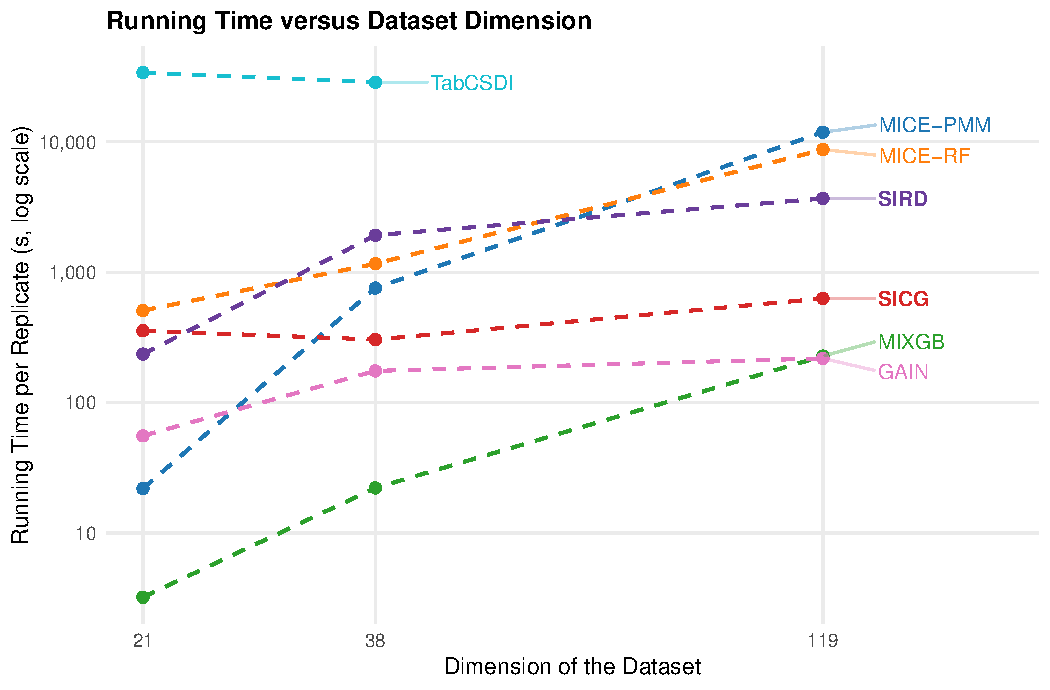
\includegraphics[width=\textwidth]{runtime_vs_dimensionality.pdf}
\caption{Median per-replicate running time in the three comparator settings, plotted against dataset dimension on a base-ten logarithmic time axis. Dashed lines join results for the same method; SICG and SIRD are shown in bold. The settings differ in more than dimension, so the connecting lines are descriptive.}
\label{fig:runtime}
\end{figure}

\subsection{Final Deployed Configurations of the Comparators}
\label{app:config_comparators}

The R methods retain their full search grids and are tuned once per setting. GAIN is also tuned over its full grid in each setting. TabCSDI holds five lower-importance diffusion and architecture parameters fixed while tuning \texttt{lr}, \texttt{batch\_size} and \texttt{featureemb} per setting. The deployed configuration is the componentwise median of the non-dominated trials, except for the survival random forest, which uses the five-trial rule in Section~\ref{sec:tuning}. In Design~III, \texttt{ntree} and \texttt{mtry} are subsequently reduced manually as described below. Table~\ref{tab:config_comparators} records the deployed values in all four settings.

\begin{table}[ht]
\centering
\caption{Deployed comparator configurations. The R methods and GAIN use their full search spaces in each setting. TabCSDI holds five lower-importance parameters fixed and tunes the remaining three. Configurations use the componentwise rule in Section~\ref{sec:tuning}; the survival random forest uses the five-trial rule, followed in Design~III by documented manual reductions to the tree count and the number of candidate variables per split. The final survival TabCSDI configuration was not carried into the simulation because of running cost.}
\label{tab:config_comparators}
\setlength{\tabcolsep}{5pt}
\begin{tabular}{llrrrr}
\toprule
Method & Parameter & Design~I & Design~II & Design~III & VCCC \\
\midrule
\multicolumn{6}{l}{\textit{\texttt{mice.impute.pmm}}} \\
 & \texttt{mincor} & 0.0775 & 0.379 & 0.053 & 0.207 \\
 & \texttt{ridge} & 0.420 & 0.498 & 0.003 & 0.439 \\
\addlinespace[2pt]
\multicolumn{6}{l}{\textit{\texttt{mice.impute.rf}}} \\
 & \texttt{ntree} & 105 & 44 & 10 & 118 \\
 & \texttt{mtry} & 6 & 13 & 63 & 23 \\
 & \texttt{nodesize} & 13 & 8 & 8 & 20 \\
 & \texttt{sampsize\_ratio} & 0.800 & 0.759 & 0.768 & 0.223 \\
\addlinespace[2pt]
\multicolumn{6}{l}{\textit{\texttt{mixgb}} (\texttt{nrounds} set separately by \texttt{mixgb\_cv})} \\
 & \texttt{gamma} & 0.445 & 0.337 & 0.334 & 0.167 \\
 & \texttt{min\_child\_weight} & 4 & 5 & 3 & 4 \\
 & \texttt{eta} & 0.105 & 0.134 & 0.093 & 0.072 \\
 & \texttt{subsample} & 0.605 & 0.650 & 0.725 & 0.687 \\
 & \texttt{max\_depth} & 4 & 4 & 2 & 6 \\
 & \texttt{colsample\_bytree} & 0.845 & 0.689 & 0.625 & 0.552 \\
\addlinespace[2pt]
\multicolumn{6}{l}{\textit{GAIN}} \\
 & \texttt{hint\_rate} & 0.63 & 0.60 & 0.65 & 0.90 \\
 & \texttt{alpha} & 330 & 100 & 200 & 350 \\
 & \texttt{beta} & 30 & 80 & 30 & 60 \\
 & \texttt{batch\_size} & 32 & 64 & 128 & 32 \\
 & \texttt{lr} & $2.5\times10^{-2}$ & $10^{-2}$ & $5\times10^{-3}$ & $10^{-2}$ \\
 & \texttt{epochs} & 9000 & 10000 & 15000 & 37000 \\
\addlinespace[2pt]
\multicolumn{6}{l}{\textit{TabCSDI} (tuned per setting)} \\
 & \texttt{lr} & $3.5\times10^{-4}$ & $2\times10^{-4}$ & $4\times10^{-4}$ & $5\times10^{-4}$ \\
 & \texttt{batch\_size} & 32 & 32 & 32 & 128 \\
 & \texttt{featureemb} & 10 & 15 & 11 & 7 \\
 & \texttt{epochs} & 3000 & 3000 & 3000 & 3000 \\
\addlinespace[2pt]
\multicolumn{6}{l}{\footnotesize TabCSDI held fixed across settings (low importance): \texttt{channels}$=128$, \texttt{nheads}$=2$,} \\
\multicolumn{6}{l}{\footnotesize \texttt{layers}$=2$, \texttt{num\_steps}$=60$, \texttt{diffusion\_embedding\_dim}$=128$.} \\
\bottomrule
\end{tabular}
\end{table}

For Simulation Design~III, the deployed random-forest values \texttt{ntree}$=10$ and \texttt{mtry}$=63$ were set manually below the values returned by the tuning search to reduce computation while retaining predictor subsampling. The tuned \texttt{nodesize}$=8$ and \texttt{sampsize\_ratio}$=0.768$ were retained.

\subsection{The Manually-Specified Comparators}
\label{app:manual_comparators}

The comparators in Table~\ref{tab:config_comparators} are the ones that carry a tuning grid. Several further comparators have no tunable hyperparameter and are defined entirely by the model they fit; this subsection specifies them setting by setting, in the notation of the corresponding technical-details section. Four estimators recur in every setting and differ only in the target model and the surrogate they use. The oracle (VAL) fits the target model on the fully validated cohort, in which the phase-two variables are known for every unit. The naive-proxy estimator (UNVAL) fits the target model on the full phase-one cohort with the error-prone surrogate in place of the validated variable. The complete-case estimator (CC) fits the target model on the validated rows only. Generalized raking (RAKING) fits a design-weighted working imputation model for the validated variable, takes the influence functions of the target-model fit as calibration variables, calibrates the phase-two design weights to them by raking, and refits the target model on the calibrated design \citep{deville1992calibration, breslow1988logistic, lumley2011complex}. The informative-sampling design adds four multiple-imputation comparators specific to it; the other three settings use only these four recurring estimators. Every multiple-imputation comparator imputes the missing values $m = 20$ times and pools the target-model fits by Rubin's rules \citep{Rubin1987}.

\paragraph{Simulation Design~I (informative sampling).} The target model is the Gaussian regression
\begin{equation}
\label{eq:appb_analysis}
Y_i = \beta_0 + \beta_X X_i + Z_i^{\top}\boldsymbol{\beta}_Z + \varepsilon_i ,
\end{equation}
with estimand $\beta_X$, where $X_i$ is the validated exposure observed only when $R_i = 1$, $\tilde{X}_i$ the error-prone surrogate used by UNVAL, $Z_i$ the recorded covariates and $W_i = 1/\pi_i$ the released design weight. Beyond VAL, UNVAL, CC and raking, four multiple-imputation comparators impute $X_i$ from the Gaussian model
\begin{equation}
\label{eq:appb_impmodel}
X_i = \boldsymbol{\alpha}^{\top}\mathbf{w}_i + \eta_i , \qquad \eta_i \sim N(0, \sigma^2), \qquad \mathbf{w}_i = (1, \tilde{X}_i, Z_i^{\top}, Y_i)^{\top},
\end{equation}
differing only in how the released weight enters:
\begin{itemize}
\item \emph{NAIVE} fits \eqref{eq:appb_impmodel} by proper Bayesian least squares on the validated rows (\texttt{imp\_gaussian} with \texttt{weighted = FALSE}), ignoring the weight; it is the standard baseline that Chapter~\ref{chap:SISL} identifies as vulnerable under informative selection.
\item \emph{NAIVE+W} adds factor-coded $W_i$ to the design vector, testing the specific extension in which the released weight enters as a categorical predictor.
\item \emph{WLMI} fits \eqref{eq:appb_impmodel} by weighted least squares with case weights $w_i = W_i/\bar{W}$ equal to the normalised design weights $(1/\pi_i)/\overline{(1/\pi)}$, and propagates the parameter uncertainty by a Bayesian bootstrap rather than a normal-theory draw \citep{Rubin1987, bartlett2020bootstrap}.
\item \emph{SISL} regresses $\log(W_i - 1)$ on flexible bases of $X_i$ and $Y_i$ to obtain a fitted inclusion function $\pi(x,V)$. It fits \eqref{eq:appb_impmodel} with
\[
f_s(x\mid V)=\frac{\pi(x,V)f_p(x\mid V)}{\mathbb E_{f_p}\{\pi(X,V)\mid V\}},
\]
and draws an unvalidated value from the normalised nonselection density
\[
f_0(x\mid V)=\frac{\{1-\pi(x,V)\}f_p(x\mid V)}{1-\mathbb E_{f_p}\{\pi(X,V)\mid V\}}
\]
\citep{pfeffermann1999parametric}. Section~\ref{sec:SISLmethod} gives the full specification.
\end{itemize}

\paragraph{Simulation Design~II (Gaussian and Binomial).} The two target models are the Gaussian systolic-blood-pressure model~\eqref{eq:appb_sbp_model} and the Binomial hypertension model~\eqref{eq:appb_htn_model}, whose exposure is the validated log-sodium intake; the error-prone dietary surrogate, the recorded average intake, plays the role of $\tilde{X}_i$ for UNVAL. Only VAL, UNVAL, CC and raking are used. Raking's working imputation model is a design-weighted Gaussian regression of the validated intake on the surrogate, the covariates and the outcome, and its calibration variables are the influence functions of the two target models.

\paragraph{Simulation Design~III (survival).} The target model is the Cox proportional-hazards model~\eqref{eq:appb_cox_true}; the error-prone surrogate laboratory and covariate values, marked with an asterisk in Appendix~\ref{app:sim2}, play the role of $\tilde{X}_i$ for UNVAL. Only VAL, UNVAL, CC and raking are used here. Raking's calibration variables are the \texttt{dfbeta} influence functions of the Cox partial-likelihood fit.

\paragraph{VCCC case study.} The three target models are the Gaussian, Binomial and Cox models of \eqref{eq:app_vccc_gauss}--\eqref{eq:app_vccc_cox}; the non-validated registry measurements play the role of $\tilde{X}_i$ for UNVAL. Only VAL, UNVAL, CC and raking are used here. Raking is applied to each target model in turn.

\section{Final Configurations for the Proposed Methods}
\label{app:proposed_config}

The comparator and proposed-method protocols differ in scope. Each comparator is tuned once per setting on the reference sample specified above. The R methods and GAIN use their full search spaces. TabCSDI uses its full space for VCCC and the reduced higher-importance space for Simulation Designs~I--III. SICG and SIRD required structural ablations, comparisons of uncertainty procedures and continuous hyperparameter searches. Repeating that full development process in every setting was computationally impractical. Their retained configurations were therefore developed on the Design~III reference setting and then reused unchanged in Simulation Designs~I and~II and the VCCC case study. This evaluates how the selected configurations transfer without per-setting retuning. It does not claim equal tuning budgets across methods or identify the fixed configurations as optimal in every setting.

Method development had two stages. The ablations in Chapters~\ref{chap:SICG} and~\ref{chap:SIRD} selected the network and loss structure, the categorical diffusion choice, classifier-free guidance and the uncertainty procedure by downstream coefficient bias, RMSE and coverage. Continuous architecture and optimisation parameters were then tuned once on a simple-random-sample replicate from Design~III. Each trial used three-fold cross-validation, masked the phase-two variables in the held-out fold, and returned $(\mathcal L_{\mathrm{data}},\mathcal L_{\mathrm{dist}})$ to a multi-objective Optuna study \citep{Akiba2019}.

The Optuna record supplies non-dominated trials and parameter-importance scores. It did not emit the deployed SICG or SIRD configuration automatically. The recorded importances were used to identify the parameters that required close attention; the trial history and marginal combined losses then guided the final values. This step included investigator judgement and should not be presented as a single automatic Pareto rule. Reproduction of the reported study uses the exact configurations in Tables~\ref{tab:config_sicg} and~\ref{tab:config_sird}. Epochs, and the SWAG learning rate where applicable, were examined in separate one-parameter sweeps. The comparator configurations continue to follow the explicit componentwise rule stated at the start of the appendix.

\subsection{SICG}

The retained configuration of SICG is the unpacked Wasserstein GAN with gradient penalty \citep{gulrajani2017improved} combined with MC-dropout multiple imputation \citep{gal2016dropout}. The ablation of Chapter~\ref{chap:SICG} set aside discriminator packing \citep{lin2018pacgan}, the auxiliary reconstruction and moment-matching losses, and the alternative SWAG \citep{maddox2019simple} and bootstrap uncertainty mechanisms, keeping the simplest generator that did not worsen interval calibration. Table~\ref{tab:tune_sicg} reports the search space over which the architecture and optimisation parameters were tuned. The importance analysis identified the generator width, the dropout rate, the learning rate and the batch size as the largest recorded contributors, together accounting for roughly nine tenths of the importance mass, and these were the parameters taken from the Pareto front, at the width of $512$, the dropout of $0.5$, the learning rate of $4 \times 10^{-4}$ and the batch size of $400$ recorded in Table~\ref{tab:config_sicg}. The remaining parameters, including the number of hidden layers, the weight decay, the Gumbel-softmax temperature \citep{jang2017categorical} and the number of discriminator steps, carried little importance and were each set one at a time from the value with the marginally lower combined loss $\mathcal{L}_{\mathrm{data}} + \mathcal{L}_{\mathrm{dist}}$ across the trial history. The discriminator-step count, for example, settled at three, between the value of one used to seed the search and the four preferred by the single lowest-loss trial. The number of training epochs was tuned separately on a categorical grid, and the shortest budget was retained because longer schedules tended to overfit the small phase-two sample. Table~\ref{tab:config_sicg} lists the final deployed configuration.

\begin{table}[ht]
\centering
\caption{Search space for SICG. The packing degree is tuned only in the packed branch of the ablation; the deployed configuration is unpacked.}
\label{tab:tune_sicg}
\begin{tabularx}{\textwidth}{lll>{\raggedright\arraybackslash}X}
\toprule
Parameter & Type & Range & Role \\
\midrule
\multicolumn{4}{l}{\textit{Stage 1: Architecture and optimisation}} \\
\texttt{hidden\_dim} & power of 2 & $\{64, \ldots, 1024\}$ &
    Generator and discriminator width. \\
\texttt{layers} & integer & $[1,\; 4]$ &
    Number of hidden layers. \\
\texttt{dropout} & continuous & $[0,\; 0.5]$ &
    Dropout rate, also the source of MC-dropout variability. \\
\texttt{lr} & log-uniform & $[10^{-4},\; 5 \times 10^{-3}]$ &
    Adam learning rate (generator and discriminator). \\
\texttt{batch\_size} & integer & $\{100, 200, \ldots, 500\}$ &
    Mini-batch size. \\
\texttt{weight\_decay} & log-uniform & $[10^{-6},\; 10^{-3}]$ &
    Adam weight decay. \\
\texttt{discriminator\_steps} & integer & $[1,\; 5]$ &
    Critic updates per generator step. \\
\texttt{tau} & continuous & $[0.1,\; 0.5]$ &
    Gumbel-softmax temperature. \\
\texttt{pack} & integer & $[2,\; 10]$ &
    Packing degree (packed branch only). \\
\midrule
\multicolumn{4}{l}{\textit{Stage 2: Training duration}} \\
\texttt{epochs} & categorical & $\{2500, \ldots, 20000\}$ &
    Number of training epochs. \\
\bottomrule
\end{tabularx}
\end{table}

\begin{table}[ht]
\centering
\caption{Final deployed configuration for SICG, reused without modification across all three simulation designs and the case study.}
\label{tab:config_sicg}
\begin{tabularx}{\textwidth}{ll>{\raggedright\arraybackslash}X}
\toprule
Parameter & Value & Role \\
\midrule
\multicolumn{3}{l}{\textit{Data processing}} \\
\texttt{normalization} & z-score & Column-wise standardisation. \\
\texttt{log} & true & Log transform of skewed variables. \\
\midrule
\multicolumn{3}{l}{\textit{Generator}} \\
\texttt{noise\_dim} & 64 & Latent noise dimension. \\
\texttt{hidden\_dim} & 512 & Hidden width. \\
\texttt{layers} & 2 & Hidden layers. \\
\texttt{dropout} & 0.5 & Dropout rate. \\
\midrule
\multicolumn{3}{l}{\textit{Discriminator}} \\
\texttt{hidden\_dim} & 512 & Hidden width. \\
\texttt{layers} & 2 & Hidden layers. \\
\texttt{pack} & 1 & Unpacked. \\
\midrule
\multicolumn{3}{l}{\textit{Multiple imputation}} \\
\texttt{m} & 20 & Number of imputations. \\
\texttt{mi\_approx} & MC-dropout & Between-imputation variance mechanism. \\
\midrule
\multicolumn{3}{l}{\textit{Training and optimisation}} \\
\texttt{epochs} & 2500 & Training epochs. \\
\texttt{batch\_size} & 400 & Mini-batch size. \\
\texttt{lr\_g}, \texttt{lr\_d} & $4 \times 10^{-4}$ &
    Adam learning rates, with $\beta = (0.5, 0.9)$. \\
\texttt{weight\_decay} & $10^{-6}$ & Adam weight decay. \\
\texttt{discriminator\_steps} & 3 & Critic updates per generator step. \\
\texttt{lambda\_gp} & 10 & Gradient-penalty weight. \\
\texttt{tau} & 0.2 & Gumbel-softmax temperature. \\
auxiliary losses & 0 &
    Reconstruction, cross-entropy, moment-matching and information losses disabled. \\
\bottomrule
\end{tabularx}
\end{table}

\subsection{SIRD}

The retained configuration of SIRD is the multinomial diffusion backbone \citep{hoogeboom2021multinomial} within the residual tabular denoising formulation \citep{kotelnikov2023tabddpm, ho2020denoising}, combined with bootstrap multiple imputation \citep{bartlett2020bootstrap}. The ablation of Chapter~\ref{chap:SIRD} discarded the analog-bits categorical encoding and did not retain classifier-free guidance \citep{ho2022classifier}, since the guided branch did not improve the downstream inferential diagnostics relative to the unguided backbone; the MC-dropout \citep{gal2016dropout} and SWAG \citep{maddox2019simple} mechanisms were examined and also set aside. Table~\ref{tab:tune_sird} reports the search space. The importance is concentrated in a single parameter to an unusual degree. The endpoint perturbation budget \texttt{sum\_scale}, which fixes the total noise variance added by the diffusion schedule, accounts for roughly one half of the importance mass, far above every other parameter. It was therefore treated as the one high-importance parameter, and its value, at the low end of its range, was read from the Pareto front. All of the remaining architecture and optimisation parameters carried low importance and were each set one at a time from the value with the marginally lower combined loss $\mathcal{L}_{\mathrm{data}} + \mathcal{L}_{\mathrm{dist}}$, as for SICG; the numeric and categorical loss weights, in particular, were of negligible importance and were held at unity. The number of diffusion steps was kept at the smallest value for which the tuning loss was still effectively flat, so that a coarser and cheaper reverse process could be used with no measurable penalty in fit. The number of training epochs was tuned on a separate categorical grid. Table~\ref{tab:config_sird} lists the final deployed configuration.

\begin{table}[ht]
\centering
\caption{Search space for SIRD. The guidance parameters are tuned only in the classifier-free-guidance branch of the ablation; the deployed configuration is unguided.}
\label{tab:tune_sird}
\begin{tabularx}{\textwidth}{lll>{\raggedright\arraybackslash}X}
\toprule
Parameter & Type & Range & Role \\
\midrule
\multicolumn{4}{l}{\textit{Stage 1: Diffusion, architecture and optimisation}} \\
\texttt{sum\_scale} & continuous & $[0.01,\; 0.25]$ &
    Terminal noise-variance budget of the schedule. \\
\texttt{num\_steps} & integer & $[20,\; 100]$ &
    Number of diffusion steps. \\
\texttt{diffusion\_embedding\_dim} & power of 2 & $\{64, 128, 256\}$ &
    Diffusion time-embedding dimension. \\
\texttt{channels} & power of 2 & $\{128, \ldots, 1024\}$ &
    Residual-block width. \\
\texttt{layers} & integer & $[2,\; 7]$ &
    Number of residual blocks. \\
\texttt{lr} & log-uniform & $[10^{-4},\; 10^{-2}]$ &
    AdamW learning rate. \\
\texttt{batch\_size} & power of 2 & $\{32, \ldots, 256\}$ &
    Mini-batch size. \\
\texttt{weight\_decay} & log-uniform & $[10^{-6},\; 10^{-3}]$ &
    AdamW weight decay. \\
\midrule
\multicolumn{4}{l}{\textit{Guidance branch (not deployed)}} \\
\texttt{cond\_drop\_prob} & continuous & $[0.05,\; 0.20]$ &
    Conditioning-dropout probability. \\
\texttt{cfg\_scale\_num}, \texttt{cfg\_scale\_cat} & continuous & $[1,\; 2]$ &
    Guidance scales for numeric and categorical variables. \\
\midrule
\multicolumn{4}{l}{\textit{Stage 2: Training duration}} \\
\texttt{epochs} & categorical & $\{2500, \ldots, 20000\}$ &
    Number of training epochs. \\
\bottomrule
\end{tabularx}
\end{table}

\begin{table}[ht]
\centering
\caption{Final deployed configuration for SIRD, reused without modification across all three simulation designs and the case study.}
\label{tab:config_sird}
\begin{tabularx}{\textwidth}{ll>{\raggedright\arraybackslash}X}
\toprule
Parameter & Value & Role \\
\midrule
\multicolumn{3}{l}{\textit{Data processing}} \\
\texttt{normalization} & z-score & Column-wise standardisation. \\
\texttt{log} & true & Log transform of skewed variables. \\
\midrule
\multicolumn{3}{l}{\textit{Diffusion}} \\
\texttt{task} & Res-N & Residual denoising target. \\
\texttt{discrete} & Multinomial & Categorical diffusion kernel. \\
\texttt{diffusion\_embedding\_dim} & 256 & Time-embedding dimension. \\
\texttt{num\_steps} & 25 & Diffusion steps. \\
\texttt{sum\_scale} & 0.01 & Terminal noise-variance budget. \\
\midrule
\multicolumn{3}{l}{\textit{Denoising network}} \\
\texttt{net} & ResNet & Residual multilayer denoiser. \\
\texttt{channels} & 256 & Residual-block width. \\
\texttt{layers} & 6 & Residual blocks. \\
\texttt{loss\_num}, \texttt{loss\_cat} & 1 & Numeric and categorical loss weights. \\
\midrule
\multicolumn{3}{l}{\textit{Multiple imputation}} \\
\texttt{m} & 20 & Number of imputations. \\
\texttt{mi\_approx} & Bootstrap & Between-imputation variance mechanism. \\
guidance & disabled & Classifier-free guidance scales set to zero. \\
\midrule
\multicolumn{3}{l}{\textit{Training and optimisation}} \\
\texttt{epochs} & 5000 & Training epochs. \\
\texttt{patience} & 2000 & Early-stopping patience. \\
\texttt{batch\_size} & 128 & Mini-batch size. \\
\texttt{lr} & $2 \times 10^{-4}$ & AdamW learning rate. \\
\texttt{weight\_decay} & $5 \times 10^{-4}$ & AdamW weight decay. \\
\bottomrule
\end{tabularx}
\end{table}

For both methods the only parameter that differs between the ablation configurations of Chapters~\ref{chap:SICG} and~\ref{chap:SIRD} and the deployed configurations above is the number of imputations, which is raised from five to twenty so that SICG and SIRD are pooled under Rubin's rules on the same number of completed datasets as the comparators \citep{Rubin1987, deng2024multiple}. The configurations in Tables~\ref{tab:config_sicg} and~\ref{tab:config_sird} are those loaded by every SICG and SIRD run reported in this thesis.

\section{Simulation Design I: Technical Details}
\label{app:infsamp}

This section documents the data-generating process and the sampling design used for the informative-sampling study of Chapter~\ref{chap:SISL}, described at a high level in Section~\ref{sec:infsamp_context}.

\subsection{Data generation}

A population of $N = 10{,}000$ individuals is generated under $500$ independent seeds. Two suppressed design variables are drawn independently and uniformly, $S_1, S_2 \in \{1, 2, 3\}$, and three recorded covariates are drawn as $Z_1, Z_2 \sim \mathcal{N}(0, 1)$ and $Z_3 \sim \mathrm{Bernoulli}(0.5)$. The stratum mean and the within-stratum standard deviations of $X$ and $Y$ are
\begin{equation}
m_{s_1 s_2} = a_{1, s_1} + a_{2, s_2}, \quad
\sigma^X_{s_1 s_2} = s_0 + s_1 (m_{s_1 s_2} - m_{\min}), \quad
\sigma^Y_{s_1 s_2} = s_0^Y + s_1^Y (m_{s_1 s_2} - m_{\min}),
\end{equation}
with $m_{\min} = \min_{s_1, s_2} m_{s_1 s_2}$. The validated measurement, the surrogate and the outcome are then generated by equations~\eqref{eq:infsamp_X}--\eqref{eq:infsamp_Y} with independent standard normal errors $\varepsilon^X_i, \tilde{\varepsilon}_i, \varepsilon^Y_i$. The parameter values are $a_1 = (-0.45,\, 0,\, 0.60)$, $a_2 = (-0.35,\, 0,\, 0.45)$, $s_0 = 0.30$, $s_1 = 0.58$, $s_0^Y = 0.30$, $s_1^Y = 0.70$, $\gamma = (0.18,\, 0.12,\, 0.14)$, $\alpha = 1.0$, $\delta = (0.40,\, 0,\, 0.50)$, $\tilde{\sigma} = 1.90$, $\beta_X = 0.48$ and $\beta = (0.30,\, 0.20,\, 0.30)$. The variance-mean coupling $s_1 > 0$ ties the within-stratum spread of $X$ to the stratum location. The surrogate has no direct $S_1$ or $S_2$ term, but it inherits information about them through $X$. Its large additional noise makes it only moderately informative about the validated measurement.

\subsection{Sampling design (\texttt{InfSamp})}

The nine combinations of $(S_1,S_2)$ are crossed with three empirical tertiles of the fully observed outcome $Y$, producing 27 joint sampling strata indexed by $h$. Under the budget $\sum_h n_h=n=500$, allocation follows $n_h\propto N_hs_h^Y$, where $N_h$ and $s_h^Y$ are the size and outcome standard deviation of joint stratum $h$. Within each joint stratum, $n_h$ individuals are selected by simple random sampling without replacement, so $\pi_i=n_h/N_h$ is positive and constant. The released data contain $(\tilde{X}_i,Z_i,Y_i)$, the selection indicator $R_i$, and the design weight $W_i=N_h/n_h=1/\pi_i$ for every individual; $X_i$ is retained only when $R_i=1$. The joint-stratum label and the variables $S_1$ and $S_2$ are not released. Thus the outcome component of the design is observed, while the stratifying variables that complete the sampling stratum remain hidden.

\section{Simulation Design II: Technical Details}
\label{app:sim1}
This section documents the data structure, measurement-error model and target models for Simulation Design~II, described in \ref{sec:sim1context}.
\subsection{Data Structure and Measurement Error Model}
\label{app:sim1_data}

Following the notation of Chapter~\ref{chap:background}, each individual $i$ has a vector of fully observed covariates $Z_i$ comprising centred age $\tilde{A}_i$, centred BMI $\tilde{B}_i$, sex indicator $F_i$, United States nativity status $U_i$, high total cholesterol indicator $C_i$, and ethnic background indicators $P_i$ (Puerto Rican) and $O_i$ (other). The error-prone phase-one dietary auxiliary vector is
\begin{equation}
    \tilde{X}_i \;=\; \bigl(
        \tilde{X}_i^{(\mathrm{Na})},\;
        \tilde{X}_i^{(\mathrm{K})},\;
        \tilde{X}_i^{(\mathrm{kcal})},\;
        \tilde{X}_i^{(\mathrm{prot})}
    \bigr)^{\top},
    \label{eq:app_phase1_aux}
\end{equation}
representing self-reported log-scale intakes of sodium, potassium, kilocalories, and protein, fully observed for all $N = 10{,}000$ individuals. The corresponding true dietary intake vector is
\begin{equation}
    X_i \;=\; \bigl(
        X_i^{(\mathrm{Na})},\;
        X_i^{(\mathrm{K})},\;
        X_i^{(\mathrm{kcal})},\;
        X_i^{(\mathrm{prot})}
    \bigr)^{\top},
    \label{eq:app_phase2_target}
\end{equation}
constituting the phase-two target variables, observed only for individuals with $R_i = 1$.

The original design of \citet{baldoni2021use} involves a three-tier measurement error structure in which the true intake $X_i$ is related to the self-reported intake $\tilde{X}_i$ through a linear Gaussian calibration model, and a biomarker $X^{**}_i = X_i + \varepsilon_i$ with $\varepsilon_i \sim \mathcal{N}(0, \sigma^2_\varepsilon)$ is additionally observed in the phase-two subsample. In the present study, the biomarker tier is removed; $X^{**}_i$ is generated but immediately discarded, and $X_i$ is treated directly as the phase-two target. The measurement error model for each component of $X_i$ retains the parametric form of \citet{baldoni2021use}. For log sodium,
\begin{equation}
    X_i^{(\mathrm{Na})} \;=\; \gamma_0
    + \gamma_1 \tilde{X}_i^{(\mathrm{Na})}
    + \gamma_2^{\top} Z_i
    + \delta_i^{(\mathrm{Na})},
    \qquad
    \delta_i^{(\mathrm{Na})} \;\sim\;
    \mathcal{N}\!\left(0,\, \sigma^2_{X,\mathrm{Na}}\right),
    \label{eq:app_meas_error_na}
\end{equation}
where $\sigma^2_{X,\mathrm{Na}} = \sigma^2_{\mathrm{Na}} - \sigma^2_{\varepsilon,\mathrm{Na}}$, with $\sigma^2_{\mathrm{Na}}$ the total variance and $\sigma^2_{\varepsilon,\mathrm{Na}}$ the biomarker error variance attenuated by a factor of $0.575$ relative to the SOLNAS estimates to ensure $\sigma^2_{X,\mathrm{Na}} > \sigma^2_{\varepsilon,\mathrm{Na}}$ \citep{baldoni2021use}. Analogous models are specified for log potassium, log kilocalories, and log protein. The coefficient $\gamma_1$ on the naive intake was inflated by a factor of $3$ for log sodium, $2$ for log potassium, and $2.5$ for log kilocalories and log protein relative to the SOLNAS estimates. This inflation was applied in \citet{baldoni2021use} to ensure that the surrogate $\tilde{X}_i$ carries sufficient information about the truth $X_i$ for the two-phase design to be effective at small sampling fractions.

\begin{table}[ht]
\centering
\caption{Gaussian linear model coefficients and variance parameters used to simulate the log-transformed true dietary intakes, reproduced from \citet{baldoni2021use}.}
\label{tab:app_meas_coef}
\begin{tabular}{lrrrr}
\hline
Coefficient & Log-sodium & Log-potassium & Log-energy & Log-protein \\
\hline
Intercept & 8.390 & 7.939 & 7.880 & 4.677 \\
Naive intake (centred) & 0.371 & 0.412 & 0.159 & 0.256 \\
Age (centred) & 0.001 & 0.006 & $-$0.001 & 0.001 \\
BMI (centred) & 0.018 & 0.012 & 0.015 & 0.017 \\
Female & $-$0.144 & $-$0.089 & $-$0.112 & $-$0.111 \\
Puerto Rican & $-$0.064 & $-$0.184 & 0.035 & $-$0.113 \\
Other background & 0.009 & 0.038 & 0.026 & 0.018 \\
Hypercholesterolaemia & $-$0.016 & $-$0.066 & $-$0.004 & $-$0.043 \\
Nativity & $-$0.086 & $-$0.036 & 0.025 & $-$0.089 \\
\hline
$\sigma^2$ & 0.220 & 0.174 & 0.021 & 0.100 \\
$\sigma^2_X$ & 0.123 & 0.089 & 0.016 & 0.055 \\
$\sigma^2_\varepsilon$ & 0.097 & 0.085 & 0.005 & 0.045 \\
\hline
\end{tabular}
\end{table}

\subsubsection{Target Outcome Models}
The original outcome model coefficients of \citet{baldoni2021use} are retained as the base specification, with two modifications. First, an interaction term $X_i^{(\mathrm{Na})} \cdot Z_i^{(\mathrm{AGE})}$ is added to both models. Second, the intercepts are recalibrated to achieve a marginal SBP mean of approximately $120\,\mathrm{mmHg}$ and a marginal hypertension prevalence of approximately $8\%$, compared to $122\,\mathrm{mmHg}$ and $10\%$ in the original. The first target model is a Gaussian model for systolic blood pressure,
\begin{align}
    Y_i^{(\mathrm{sbp})} \;=\; \beta_0
    &+ \beta_1 Z_i^{(\mathrm{AGE})}
    + \beta_2 Z_i^{(\mathrm{BMI})}
    + \beta_3 X_i^{(\mathrm{Na})}
    + \beta_4 Z_i^{(\mathrm{CHOL})}
    + \beta_5 Z_i^{(\mathrm{BORN})}
    + \beta_6 Z_i^{(\mathrm{SEX})} \nonumber \\
    &+ \beta_7 Z_i^{(\mathrm{PR})}
    + \beta_8 Z_i^{(\mathrm{OTH})}
    + \beta_9 \bigl(X_i^{(\mathrm{Na})} \cdot Z_i^{(\mathrm{AGE})}\bigr)
    + \varepsilon_i,
    \label{eq:appb_sbp_model}
\end{align}
with $\varepsilon_i \sim \mathcal{N}(0,\, \sigma^2)$, $\sigma^2 = 145.740$, and true interaction coefficient $\beta_9 = 0.15$. The remaining coefficients are given in Table~\ref{tab:app_outcome_coef}. The second target model is a Binomial model for hypertension status $Y_i^{(\mathrm{htn})} \in \{0,1\}$,
\begin{align}
    \log \frac{\Pr(Y_i^{(\mathrm{htn})} = 1)}{%
              1 - \Pr(Y_i^{(\mathrm{htn})} = 1)}
    \;=\; \alpha_0
    &+ \alpha_1 Z_i^{(\mathrm{AGE})}
    + \alpha_2 Z_i^{(\mathrm{BMI})}
    + \alpha_3 X_i^{(\mathrm{Na})}\nonumber \\
    &+ \alpha_4 Z_i^{(\mathrm{CHOL})}
    + \alpha_5 Z_i^{(\mathrm{BORN})}
    + \alpha_6 Z_i^{(\mathrm{SEX})}\nonumber \\
    &+ \alpha_7 Z_i^{(\mathrm{PR})}
    + \alpha_8 Z_i^{(\mathrm{OTH})}
    + \alpha_9 \bigl(X_i^{(\mathrm{Na})} \cdot Z_i^{(\mathrm{AGE})}\bigr),
    \label{eq:appb_htn_model}
\end{align}
with true interaction coefficient $\alpha_9 = 0.005$. The remaining coefficients are given in Table~\ref{tab:app_outcome_coef}.

\begin{table}[ht]
\centering
\caption{Outcome model coefficients used in the present simulation study. Base coefficients are reproduced from \citet{baldoni2021use}; intercepts are recalibrated and interaction coefficients are added in the present study.}
\label{tab:app_outcome_coef}
\begin{tabular}{lrr}
\hline
Coefficient & SBP ($\hat{\beta}$) & Hypertension ($\hat{\alpha}$) \\
\hline
Intercept (recalibrated) & 120.000 (approx.) & $-$2.340 (approx.) \\
Log-sodium (centred) & 27.473 & 1.439 \\
Age (centred) & 0.406 & 0.087 \\
BMI (centred) & 0.170 & 0.056 \\
Female & $-$8.932 & $-$0.120 \\
Puerto Rican & $-$1.670 & $-$0.175 \\
Other background & $-$2.322 & $-$0.845 \\
Hypercholesterolaemia & 1.611 & 0.379 \\
Nativity & $-$0.564 & $-$0.220 \\
Interaction (Na $\times$ Age) & 0.150 & 0.005 \\
$\sigma^2$ & 145.740 & --- \\
\hline
\end{tabular}
\end{table}

\subsection{Sampling Designs}
\label{app:sim1_sampling}

Seven sampling designs are applied to each of the $500$ simulated populations to draw the phase-two validation sample of size $n = 500$. For each design, the selection indicator $R_i \in \{0,1\}$ is defined, $X_i$ is masked for all individuals with $R_i = 0$, and sampling weights $W_i$ are assigned according to the design. The probability designs (\texttt{SRS}, \texttt{Neyman-ODS}, \texttt{Neyman-IF}) admit a positive inclusion probability $\pi_i$ for every unit and carry the design weight $W_i = 1/\pi_i$, which the design-based estimators require; the tail-based designs (\texttt{RS}, \texttt{WRS}, \texttt{SFS}, \texttt{ODS-Tail}) select units deterministically from the extremes of a phase-one score and do not define a positive inclusion probability for every unit, so no design weights are available for them and they are analysed unweighted. Unless otherwise stated, all $W_i = 1$.

\subsubsection{Design 1: Simple Random Sampling (\texttt{SRS})}

Each individual is selected independently with equal inclusion probability $\pi_i = n/N = 0.05$, so the design weight $W_i = 1/\pi_i = N/n = 20$ is constant across units and the weighted analysis coincides with the unweighted one. \texttt{SRS} serves as the na\"ive unweighted baseline and represents the most common validation design used in measurement-error practice \citep{amorim2021two}.

\subsubsection{Design 2: Residual Sampling (\texttt{RS})}

A phase-one linear model for $Y^{(\mathrm{sbp})}$ is fitted using $Z_i$ and $\tilde{X}_i$ jointly. Residuals $\hat{e}_i$ are computed for all $N$ individuals. The $n/2$ individuals with the most extreme positive residuals and the $n/2$ with the most extreme negative residuals are selected deterministically.

For model-based estimators, residual sampling directs validation towards observations whose outcomes are poorly predicted by the phase-one covariates. \citet[Sections~3 and~5]{amorim2021two} show that it performs similarly to the locally optimal weighted-residual design when $\beta$ is close to zero and $\operatorname{Var}(X\mid X^*,Z)$ is constant across $Z$.

\subsubsection{Design 3: Weighted Residual Sampling (\texttt{WRS})}

\citet{tao2019optimal} derived the optimal model-based design under the local alternative $\beta = o(1)$: phase-two selection should maximise $(Y_i - \mu(Z_i))^2 \operatorname{Var}(X_i \mid X^*_i, Z_i)$, where $\mu(Z_i)$ is the linear predictor from a regression of $Y$ on $Z$ alone. The factor $\operatorname{Var}(X \mid X^*, Z)$ up-weights individuals whose error-prone measurements are least informative about the truth; when this variance is approximately constant across covariate levels, \texttt{WRS} reduces to residual sampling \citep[Section~3.1]{amorim2021two}. Because $\operatorname{Var}(X \mid X^*, Z)$ is unknown from phase-one data alone, a pilot subsample of size $n_{\mathrm{pilot}} = \lfloor 0.1 \times n \rfloor = 50$ is drawn by simple random sampling from the $N$ phase-one individuals. A pilot regression of $X^{(\mathrm{Na})}$ on $Z_i$ and $\tilde{X}_i$ is fitted to this subsample, yielding the residual standard deviation $\hat{\sigma}_{\mathrm{pilot}}$. For the remaining $N - n_{\mathrm{pilot}}$ individuals, a phase-one model for $Y^{(\mathrm{sbp})}$ on $Z_i$ alone is fitted and its residuals $\hat{e}^*_i$ are scaled to form $\tilde{e}_i = \hat{e}^*_i \cdot \hat{\sigma}_{\mathrm{pilot}}$. The remaining $n - n_{\mathrm{pilot}}$ individuals are drawn from the tails of $\tilde{e}_i$, and the pilot subsample is combined to complete the phase-two cohort.

\subsubsection{Design 4: Score Function Sampling (\texttt{SFS})}

A phase-one linear model for $Y^{(\mathrm{sbp})}$ is fitted on $Z_i$ only, excluding $\tilde{X}_i$. The empirical score contribution for the sodium coefficient is approximated as $s_i = \hat{e}_i \cdot \tilde{X}_i^{(\mathrm{Na})}$, where $\hat{e}_i$ is the model residual. The $n/2$ individuals with the most extreme positive and negative values of $s_i$ are selected.

\citet{amorim2021two} propose \texttt{SFS} as a practical alternative to \texttt{WRS}: it avoids the need for a pilot sample or prior knowledge of $\operatorname{Var}(X \mid X^*, Z)$ by substituting the error-prone covariate $X^*$ directly into the score expression. \texttt{SFS} therefore selects individuals using the product of the phase-one residual and the surrogate covariate. Simulations in \citet[Table~1]{amorim2021two} show that \texttt{SFS} outperforms \texttt{RS} and \texttt{WRS} when $\beta$ deviates substantially from zero and $X^*$ is a fair surrogate for $X$.

\subsubsection{Design 5: Outcome-Dependent Sampling by Tails (\texttt{ODS-Tail})}

The $n/2$ individuals at the lower extreme and the $n/2$ at the upper extreme of the $Y^{(\mathrm{sbp})}$ distribution are deterministically selected. Outcome-dependent sampling exploits the fact that subjects in the tails of the outcome distribution exert greater influence on the regression parameter; by oversampling them, one expects to increase efficiency for model-based estimators \citep{zhou2002semiparametric, amorim2021two}.

\subsubsection{Design 6: Outcome-Dependent Sampling by Neyman Allocation (\texttt{Neyman-ODS})}

The distribution of $Y^{(\mathrm{sbp})}$ is partitioned into three strata at the 19th and 81st empirical percentiles. Within stratum $k$, the phase-two allocation is $n_k \propto N_k \hat{S}_k$, where $N_k$ is the stratum size and $\hat{S}_k$ is the within-stratum standard deviation of the phase-one sodium proxy $\tilde{X}_i^{(\mathrm{Na})}$. For this allocation variable, the Neyman criterion minimises the design variance of its Horvitz--Thompson total at a fixed sample size \citep{neyman1938contribution}. It is an auxiliary-variable Neyman allocation; Design~7 instead bases the allocation on an approximate influence function for a regression coefficient. Sampling weights are set to $W_i = N_k / n_k$ for all individuals in stratum~$k$ \citep{Weaver2005, lumley2011connections}.

\subsubsection{Design 7: Influence Function Sampling by Neyman Allocation (\texttt{Neyman-IF})}

The same three $Y^{(\mathrm{sbp})}$-based strata from Design~6 are retained. For each individual $i$, the approximate influence $\mathrm{h}_i(\hat{\beta})$ on the $\tilde{A}$ coefficient is computed via the \texttt{dfbeta} approximation applied to the phase-one model for $Y^{(\mathrm{sbp})}$ augmented by $\tilde{X}_i^{(\mathrm{Na})}$ and its interaction with $\tilde{A}_i$. The Neyman allocation within strata is driven by the within-stratum standard deviation of $\mathrm{h}_i(\hat{\beta})$.

\citet[Section~4.1]{amorim2021two} prove that for IPW estimators the optimal phase-two allocation from stratum~$k$ satisfies $n_k / n = N_k s_k / \sum_{k'} N_{k'} s_{k'}$, where $s_k$ is the standard deviation of the influence function for $\hat{\beta}$ within stratum~$k$. Because $\hat{\beta}_w$ is asymptotically equivalent to a sum of influence functions \citep[eq.~10]{amorim2021two}, this result is the direct translation of classical Neyman allocation from the population-total setting to two-phase regression \citep{lumley2011connections, mcisaac2014response}. The influence function is approximated by replacing the unobserved $X_i$ with the error-prone $\tilde{X}_i$; \citet{amorim2021two} recommend that this approximation be highly correlated with the true influence function (following the $r \geq 0.90$ rule of thumb of \citealt{sarndal1992model}). Sampling weights are set to $W_i = N_k / n_k$.

For the two stratified probability designs, the realised per-stratum sampling fractions, averaged over the $500$ replicates, show how the fixed budget of $n = 500$ is distributed across strata. The three $Y^{(\mathrm{sbp})}$ strata, cut at the 19th and 81st percentiles with sizes $N_k \approx 1900$, $6200$ and $1900$, receive sampling fractions $n_k/N_k$ of approximately $0.051$, $0.050$ and $0.048$ under \texttt{Neyman-ODS}, so that this outcome-stratified allocation is close to proportional; under \texttt{Neyman-IF} the same strata receive approximately $0.070$, $0.038$ and $0.069$, concentrating the validation budget in the two outer strata, where the influence-function spread is largest. Under \texttt{SRS} every unit is sampled at the common fraction $0.05$.


\section{Simulation Design III: Technical Details}
\label{app:sim2}
This section documents the electronic-health-record parameter estimates, data structure and target model for Simulation Design~III, described in \ref{sec:sim2context}.
\subsection{Empirical Parameter Estimation from EHR Data}
\label{app:sim2_ehr}

The clinical laboratory parameters used in this simulation are estimated from a retrospective electronic health record cohort comprising $530{,}165$ emergency department presentations across two New Zealand metropolitan hospitals (North Shore Hospital and Waitakere Hospital) between July 2016 and June 2021. Key characteristics of the cohort include a mean age of $52.6$ years (SD $21.7$), $54.1\%$ female, and a hospital admission rate of approximately $40\%$.

For each laboratory panel, a race- and sex-stratified covariance matrix $\hat{\Sigma}$ is estimated from the EHR data using pairwise complete observations, then projected to the nearest positive semi-definite matrix. The panels and their constituent variables are: renal (creatinine, urea, potassium, sodium, chloride, bicarbonate, calcium, magnesium, phosphate); hepatic (aspartate aminotransferase [AST], alanine aminotransferase [ALT], alkaline phosphatase [ALP], gamma-glutamyl transferase [GGT], bilirubin, albumin, globulin, total protein); haematology (haemoglobin [Hb], haematocrit [HCT], red and white blood cell counts [RBC and WBC], platelet count, mean corpuscular volume [MCV], red cell distribution width [RDW], neutrophils, lymphocytes, monocytes, eosinophils, basophils); lipids (triglycerides, high-density lipoprotein [HDL], low-density lipoprotein [LDL]); diabetic markers (glucose, fasting glucose, glycated haemoglobin [HbA1c], insulin); and vital signs (systolic blood pressure [SBP], temperature, heart rate, peripheral oxygen saturation [SpO2]).

For each variable within each panel, a generalised linear model regressing the variable on sex, race, age, BMI, smoking status, and medication count is fitted to the EHR data. Only predictors significant at $p < 0.05$ in the multivariable model are retained; non-significant predictors are set to zero in the simulation. To protect data privacy, independent Gaussian noise $\mathcal{N}(0, 0.05^2)$ is added to each race-specific regression coefficient before use in the simulation. The complete set of estimated coefficients and covariance matrices is fixed across all $500$ simulation replicates.

\subsection{Population Variable Generation}
\label{app:sim2_popgen}

Each simulated population of $N = 20{,}000$ individuals is generated sequentially in the order shown in Table~\ref{tab:app_sim2_overview}. All continuous laboratory outcomes are generated on the log scale and back-transformed via $\exp(\cdot) - 1$ before use. Multivariate panels are drawn jointly from a multivariate Gaussian distribution with empirically estimated covariance matrix $\hat{\Sigma}$ and conditional mean $\boldsymbol{\mu}_i = \hat{\boldsymbol{\gamma}}^{\top}\mathbf{c}_i$.

\begin{table}[ht]
\centering
\caption{Variable generation order, distribution family, predictor set, and back-transformation for each variable or group.}
\label{tab:app_sim2_overview}
\small
\begin{tabular}{p{3.2cm}p{3.2cm}p{4.9cm}p{1.5cm}}
\hline
\textbf{Variable / Group} & \textbf{Distribution} &
\textbf{Predictors} & \textbf{Transf.} \\
\hline
AGE & Trunc.\ Normal$(62,10^2)$, $[25,90]$ & None & No \\
SEX & Bernoulli$(0.55)$ & None & No \\
RACE & Multinomial & None & No \\
INSURANCE & Bernoulli$(0.70)$ & None & No \\
REGION & Categorical (20) & None & No \\
URBAN & Derived & REGION & No \\
INCOME & Categorical (5) & None & No \\
EDU & Poisson$(4)+6$ & None & No \\
15 SNP genotypes & Binomial, Hardy--Weinberg equilibrium & Race-specific minor allele frequencies and linkage disequilibrium & No \\
HEIGHT & Normal & SEX, rs11708067 & No \\
SMOKE & Multinomial logit & AGE, SEX, RACE & No \\
EXER & Multinomial logit & AGE, SEX, RACE, SMOKE & No \\
ALC & Multinomial logit & AGE, SEX, RACE, SMOKE, EXER & No \\
BMI & Log-Normal & SEX, SMOKE, RACE, AGE, 4 SNPs$^a$ & Yes \\
MARRIAGE & Multinomial logit & AGE, SEX, RACE, BMI & No \\
MED\_Count & Poisson log-linear & SEX, SMOKE, RACE, AGE, BMI & No \\
RENAL (9 vars) & Multiv. normal & Standard set$^b$ & Yes \\
LIPIDS (3 vars) & Multiv. normal & Standard set$^b$ & Yes \\
HEMA (12 vars) & Multiv. normal & Standard set$^b$ & Yes \\
NUTRIENTS (4 vars) & Multiv. normal & AGE, SEX, BMI, RACE & Yes \\
LIVER (8 vars) & Multiv. normal & Standard set$^b$ & Yes \\
DIABETE (4 vars) & Multiv. normal & Variable-specific$^c$ & Yes \\
FERRITIN & Log-Normal & SEX, SMOKE, RACE, AGE, MED\_Count & Yes \\
VITALS (4 vars) & Multiv. normal & Variable-specific$^c$ & Yes \\
WEIGHT & Derived & BMI, HEIGHT & No \\
Estimated glomerular filtration rate (eGFR) & Chronic Kidney Disease Epidemiology Collaboration (CKD-EPI) formula & Creatinine, AGE, SEX & No \\
\hline
\multicolumn{4}{l}{$^a$ SNPs: rs10811661, rs11708067, rs4506565, rs5219.} \\
\multicolumn{4}{l}{$^b$ Standard set: SEX, SMOKE, RACE, AGE, BMI, MED\_Count; some variables exclude} \\
\multicolumn{4}{l}{\phantom{$^b$} certain predictors; see Tables~\ref{tab:app_coef_renal}--\ref{tab:app_coef_liver}.} \\
\multicolumn{4}{l}{$^c$ Variable-specific predictors; see Tables~\ref{tab:app_coef_vitals} and~\ref{tab:app_coef_diabete}.} \\
\end{tabular}
\end{table}

\subsection{Regression Coefficients}
\label{app:sim2_coef}

The multivariate-normal blocks listed above, namely RENAL, LIPIDS, HEMA, NUTRIENTS, LIVER, DIABETE, and VITALS, are panels of correlated clinical measurements generated jointly and named for the physiological system they represent; for example, the DIABETE panel collects the glycaemic markers (non-fasting and fasting glucose, glycated haemoglobin, and insulin) and the LIPIDS panel the serum lipids (triglyceride, HDL, and LDL). Tables~\ref{tab:app_coef_scalar}--\ref{tab:app_coef_diabete} report the regression coefficients $\hat{\boldsymbol{\gamma}}$ for each variable group, with predictors as rows and outcome variables as columns. RACE categories are coded relative to European (EUR): RACE2~=~African (AFR), RACE3~=~Admixed American (AMR), RACE4~=~South Asian (SAS), and RACE5~=~East Asian (EAS). SMOKE categories are relative to Current Smoker. All SNP coefficients represent the per-allele additive effect. A dash (---) indicates the predictor was excluded at $p < 0.05$ in the EHR regression.

\begin{table}[ht]
\centering
\caption{Coefficients for scalar variables. Columns give (1)~height, (2)~body mass index on the log scale, (3)~medication count under a Poisson log-linear model, and (4)~ferritin on the log scale.}
\label{tab:app_coef_scalar}
\small
\begin{tabular}{lrrrr}
\hline
\textbf{Predictor} & \textbf{(1)} & \textbf{(2)} &
\textbf{(3)} & \textbf{(4)} \\
\hline
Intercept        & 162.000 &  3.383 & $-$0.334 &  3.073 \\
SEX              &  13.000 &  0.009 & $-$0.126 &  0.625 \\
SMOKE\_Ex        &     --- &  0.063 & $-$0.368 & $-$0.086 \\
SMOKE\_Nev       &     --- &  0.038 & $-$0.495 & $-$0.053 \\
RACE2 (AFR)      &     --- &  0.081 &    0.363 &  0.032 \\
RACE3 (AMR)      &     --- &  0.242 &    0.114 &  0.228 \\
RACE4 (SAS)      &     --- &  0.032 & $-$0.134 & $-$0.124 \\
RACE5 (EAS)      &     --- & $-$0.200 & $-$0.408 &  0.221 \\
AGE              &     --- & $-$0.0018 &  0.0180 &  0.0120 \\
BMI              &     --- &    --- &    0.693 &    --- \\
MED\_Count       &     --- &    --- &      --- & $-$0.001 \\
rs11708067       &   0.015 &  0.055 &      --- &    --- \\
rs10811661       &     --- &  0.027 &      --- &    --- \\
rs4506565        &     --- &  0.011 &      --- &    --- \\
rs5219           &     --- &  0.012 &      --- &    --- \\
\hline
\end{tabular}
\end{table}

\begin{table}[ht]
\centering
\caption{Coefficients for the vital-sign measurements on the log scale. Columns give (1)~systolic blood pressure, (2)~temperature, (3)~heart rate, and (4)~oxygen saturation.}
\label{tab:app_coef_vitals}
\small
\begin{tabular}{lrrrr}
\hline
\textbf{Predictor} & \textbf{(1)} & \textbf{(2)} & \textbf{(3)} & \textbf{(4)} \\
\hline
Intercept    &  4.3936 &  3.6311 &  4.3458 &  4.6071 \\
SEX          &  0.0083 & $-$0.0012 &     --- &  0.0003 \\
SMOKE\_Ex    & $-$0.0236 &  0.0006 & $-$0.0068 &  0.0002 \\
SMOKE\_Nev   & $-$0.0096 &  0.0013 & $-$0.0053 &  0.0019 \\
RACE2 (AFR)  & $-$0.0334 &  0.0346 & $-$0.0812 &  0.0308 \\
RACE3 (AMR)  & $-$0.0504 &  0.0520 & $-$0.0089 &  0.0683 \\
RACE4 (SAS)  &  0.0557 &  0.0918 &  0.0285 & $-$0.0078 \\
RACE5 (EAS)  & $-$0.0414 & $-$0.0400 &  0.0479 &  0.0895 \\
AGE          &     --- & $-$0.0000224 & $-$0.0006 & $-$0.0001 \\
BMI          &  0.0876 &  0.0009 &     --- & $-$0.0038 \\
MED\_Count   & $-$0.0006 &  0.0000086 &  0.0001 & $-$0.0000245 \\
rs5219       &  0.3200 &     --- &     --- &     --- \\
rs7754840    &  0.1800 &     --- &     --- &     --- \\
rs7756992    &  0.2075 &     --- &     --- &     --- \\
\hline
\end{tabular}
\end{table}

\begin{landscape}
\begin{table}[ht]
\centering
\caption{Coefficients for the renal measurements on the log scale. Columns give (1)~creatinine, (2)~urea, (3)~potassium, (4)~sodium, (5)~chloride, (6)~bicarbonate, (7)~calcium, (8)~magnesium, and (9)~phosphate. Dashes indicate a predictor excluded at $p < 0.05$.}
\label{tab:app_coef_renal}
\resizebox{\linewidth}{!}{%
\begin{tabular}{lrrrrrrrrr}
\hline
\textbf{Predictor} & \textbf{(1)} & \textbf{(2)} &
\textbf{(3)} & \textbf{(4)} & \textbf{(5)} & \textbf{(6)} &
\textbf{(7)} & \textbf{(8)} & \textbf{(9)} \\
\hline
Intercept    &  2.8712 &  0.3175 &  1.4837 &  4.9161 &  4.6337
             &  3.1565 &  1.1792 &  0.6138 &  0.6992 \\
SEX          &  0.2924 &  0.1955 &  0.0186 &  0.0018 & $-$0.0032
             &  0.0056 & $-$0.0061 &  0.0102 &     --- \\
SMOKE\_Ex    &  0.1065 &  0.1982 &  0.0057 &     --- &     ---
             & $-$0.0078 &  0.0022 &  0.0113 &  0.0187 \\
SMOKE\_Nev   &  0.0850 &  0.1580 &  0.0044 &     --- &     ---
             & $-$0.0083 &  0.0052 &  0.0193 &  0.0084 \\
RACE2 (AFR)  &  0.2296 &  0.3067 &  0.0439 & $-$0.0044 &  0.0321
             & $-$0.0901 & $-$0.0565 &  0.0141 &  0.0255 \\
RACE3 (AMR)  &  0.2816 &  0.3517 &  0.0086 &  0.1157 & $-$0.0639
             & $-$0.1041 &  0.0801 &  0.0710 &  0.1331 \\
RACE4 (SAS)  &  0.1041 &  0.1591 & $-$0.0036 &  0.0277 & $-$0.0559
             & $-$0.0125 &  0.0307 &  0.0460 & $-$0.0291 \\
RACE5 (EAS)  &  0.0138 &  0.1053 & $-$0.0435 & $-$0.0068 &  0.0210
             & $-$0.1142 &  0.0196 & $-$0.0179 &  0.0268 \\
AGE          &  0.0061 &  0.0110 &  0.0008 & $-$0.0002 & $-$0.0003
             &  0.0003 & $-$0.0001 & $-$0.0002 &     --- \\
BMI          &  0.2091 &  0.1880 &  0.0188 &  0.0080 &  0.0062
             &  0.0123 &  0.0039 & $-$0.0086 &     --- \\
MED\_Count   &  0.0025 &  0.0016 &  0.0002 & $-$0.0001 & $-$0.0001
             &  0.0002 &  0.0001 &     --- &  0.0007 \\
\hline
\end{tabular}}
\end{table}
\end{landscape}

\begin{table}[ht]
\centering
\caption{Coefficients for the lipid measurements on the log scale. Columns give (1)~triglyceride, (2)~high-density lipoprotein cholesterol, and (3)~low-density lipoprotein cholesterol.}
\label{tab:app_coef_lipids}
\small
\begin{tabular}{lrrr}
\hline
\textbf{Predictor} & \textbf{(1)} & \textbf{(2)} & \textbf{(3)} \\
\hline
Intercept    & $-$0.089 &  1.479 &  1.532 \\
SEX          &    0.041 & $-$0.100 & $-$0.055 \\
SMOKE\_Ex    & $-$0.029 &  0.000 & $-$0.031 \\
SMOKE\_Nev   & $-$0.065 &  0.012 & $-$0.003 \\
RACE2 (AFR)  & $-$0.040 & $-$0.025 &  0.047 \\
RACE3 (AMR)  & $-$0.053 & $-$0.056 & $-$0.108 \\
RACE4 (SAS)  &    0.055 & $-$0.063 &  0.012 \\
RACE5 (EAS)  &    0.098 &  0.010 & $-$0.133 \\
AGE          & $-$0.001 &  0.000 & $-$0.003 \\
BMI          &    0.317 & $-$0.154 &    --- \\
MED\_Count   &    0.001 & $-$0.000 & $-$0.001 \\
rs17036101   &    0.032 &    --- &    --- \\
rs7756992    &      --- &    --- &  0.020 \\
\hline
\end{tabular}
\end{table}

\begin{table}[ht]
\centering
\caption{Coefficients for the glycaemic measurements on the log scale. Columns give (1)~glucose, (2)~fasting glucose, (3)~glycated haemoglobin, and (4)~insulin. Insulin has one retained predictor, rs11708067.}
\label{tab:app_coef_diabete}
\small
\begin{tabular}{lrrrr}
\hline
\textbf{Predictor} & \textbf{(1)} & \textbf{(2)} & \textbf{(3)} & \textbf{(4)} \\
\hline
Intercept    &  1.1823 &  0.9513 &  2.5740 &  3.0134 \\
SEX          &  0.0507 &     --- &  0.0613 &     --- \\
SMOKE\_Ex    &     --- &     --- & $-$0.0125 &     --- \\
SMOKE\_Nev   &     --- &     --- & $-$0.0228 &     --- \\
RACE2 (AFR)  &  0.0506 &     --- &  0.1534 &     --- \\
RACE3 (AMR)  &  0.1770 &     --- &  0.1914 &     --- \\
RACE4 (SAS)  &  0.1484 &     --- &  0.0775 &     --- \\
RACE5 (EAS)  &  0.0782 &     --- &  0.0253 &     --- \\
AGE          &  0.0033 &     --- &  0.0035 &     --- \\
BMI          &  0.1546 &  0.2882 &  0.2575 &     --- \\
MED\_Count   &  0.0008 &     --- &  0.0012 &     --- \\
rs7756992    &  0.0340 &     --- &     --- &     --- \\
rs10811661   &     --- &  0.0297 &  0.0918 &     --- \\
rs11708067   &     --- &  0.0327 &  0.0523 &  0.0135 \\
rs4506565    &     --- &  0.0229 &     --- &     --- \\
\hline
\end{tabular}
\end{table}

\begin{table}[ht]
\centering
\caption{Coefficients for the dietary-intake measurements on the log scale. Columns give (1)~sodium intake, (2)~potassium intake, (3)~energy intake, and (4)~protein intake.}
\label{tab:app_coef_nutrients}
\small
\begin{tabular}{lrrrr}
\hline
\textbf{Predictor} & \textbf{(1)} & \textbf{(2)} & \textbf{(3)} & \textbf{(4)} \\
\hline
Intercept    &    7.660 &    7.200 &    7.400 &    4.000 \\
AGE          & $-$0.00084 &  0.00750 & $-$0.00256 &  0.00046 \\
SEX          &    0.270 &    0.177 &    0.160 &    0.187 \\
BMI          &    0.018 &    0.010 &    0.014 &    0.017 \\
RACE2 (AFR)  &    0.009 &    0.040 &    0.200 &    0.020 \\
RACE3 (AMR)  & $-$0.100 & $-$0.080 & $-$0.400 & $-$0.130 \\
RACE4 (SAS)  & $-$0.150 & $-$0.120 & $-$0.600 & $-$0.140 \\
RACE5 (EAS)  &    0.030 &    0.020 &    0.120 &    0.100 \\
\hline
\end{tabular}
\end{table}

\begin{landscape}
\begin{table}[ht]
\centering
\caption{Coefficients for the liver measurements on the log scale. Columns give (1)~aspartate aminotransferase, (2)~alanine aminotransferase, (3)~alkaline phosphatase, (4)~gamma-glutamyl transferase, (5)~bilirubin, (6)~albumin, (7)~globulin, and (8)~total protein. Dashes indicate a predictor excluded at $p < 0.05$.}
\label{tab:app_coef_liver}
\resizebox{\linewidth}{!}{%
\begin{tabular}{lrrrrrrrr}
\hline
\textbf{Predictor} & \textbf{(1)} & \textbf{(2)} & \textbf{(3)} & \textbf{(4)} &
\textbf{(5)} & \textbf{(6)} & \textbf{(7)} & \textbf{(8)} \\
\hline
Intercept    &  3.325 &  2.345 &  4.074 &  1.637
             &  1.823 &  3.731 &  3.304 &  4.204 \\
SEX          &  0.106 &  0.173 &  0.034 &  0.265
             &  0.207 &    --- &    --- &  0.002 \\
SMOKE\_Ex    & $-$0.107 & $-$0.027 & $-$0.031 & $-$0.080
             &  0.061 & $-$0.011 & $-$0.004 & $-$0.003 \\
SMOKE\_Nev   & $-$0.041 &  0.009 & $-$0.035 & $-$0.127
             &  0.093 &  0.005 & $-$0.013 & $-$0.002 \\
RACE2 (AFR)  &  0.007 & $-$0.075 &  0.057 &  0.179
             &  0.150 & $-$0.118 &  0.005 &  0.039 \\
RACE3 (AMR)  &  0.069 &  0.024 &  0.039 &  0.103
             &  0.168 & $-$0.103 &  0.148 &  0.044 \\
RACE4 (SAS)  & $-$0.009 &  0.034 & $-$0.001 &  0.207
             &  0.026 & $-$0.040 & $-$0.011 &  0.070 \\
RACE5 (EAS)  &  0.075 &  0.120 &  0.014 &  0.304
             &  0.124 &  0.022 &  0.097 & $-$0.063 \\
AGE          &  0.0022 & $-$0.0041 &  0.0047 &  0.0063
             &  0.0039 & $-$0.0028 & $-$0.0001 & $-$0.0013 \\
BMI          &    --- &  0.312 &  0.042 &  0.419
             & $-$0.039 &    --- &  0.092 &  0.042 \\
MED\_Count   & $-$0.001 & $-$0.000 &  0.001 &  0.002
             & $-$0.001 & $-$0.000 &  0.000 & $-$0.000 \\
rs11708067   &    --- &  0.032 &  0.015 &    ---
             &    --- &    --- &    --- &    --- \\
rs17036101   &    --- &  0.045 &    --- &    ---
             &    --- &  0.050 &    --- &    --- \\
rs4506565    &    --- &    --- &    --- &    ---
             &    --- &  0.016 &    --- &    --- \\
\hline
\end{tabular}}
\end{table}
\end{landscape}


\subsection{Residual Variances and Covariance Matrices}
\label{app:sim2_sigma}

For univariate variables the residual standard deviations are $\hat{\sigma}_{\mathrm{HEIGHT}} = 7.0\,\mathrm{cm}$, $\hat{\sigma}_{\mathrm{BMI}} = 0.063$ (log scale), and $\hat{\sigma}_{\mathrm{FERRITIN}} = 1.350$ (log scale). For multivariate panels the full empirical covariance matrices $\hat{\Sigma}$ are too large to reproduce in full; Table~\ref{tab:app_sigma_diag} reports the diagonal entries (residual variances on the log scale). The complete off-diagonal covariance structure is available in the simulation codebase.

\begin{center}
\small
\begin{longtable}{llr}
\caption{Diagonal entries (residual variances, log scale) of $\hat{\Sigma}$ for each multivariate panel.}\label{tab:app_sigma_diag}\\
\hline
\textbf{Panel} & \textbf{Variable} & \textbf{Residual variance} \\
\hline
\endfirsthead
\multicolumn{3}{c}{\tablename~\thetable\ (continued)} \\
\hline
\textbf{Panel} & \textbf{Variable} & \textbf{Residual variance} \\
\hline
\endhead
\hline
\endfoot
VITALS      & SBP                & 0.10950  \\
            & Temperature        & 0.000219 \\
            & Heart rate         & 0.01770  \\
            & SpO2               & 0.000247 \\
\hline
RENAL       & Creatinine         & 0.34460  \\
            & Urea               & 0.42530  \\
            & Potassium          & 0.01310  \\
            & Sodium             & 0.000849 \\
            & Chloride           & 0.002610 \\
            & Bicarbonate        & 0.02700  \\
            & Calcium            & 0.003140 \\
            & Magnesium          & 0.006930 \\
            & Phosphate          & 0.04590  \\
\hline
LIPIDS      & Triglyceride       & 0.12490  \\
            & HDL                & 0.03360  \\
            & LDL                & 0.08770  \\
\hline
HEMA        & Hb                 & 0.03650  \\
            & HCT                & 0.002070 \\
            & RBC                & 0.02340  \\
            & WBC                & 0.15100  \\
            & Platelet           & 0.20680  \\
            & MCV                & 0.005860 \\
            & RDW                & 0.01640  \\
            & Neutrophils        & 0.21820  \\
            & Lymphocytes        & 0.10550  \\
            & Monocytes          & 0.03750  \\
            & Eosinophils        & 0.02310  \\
            & Basophils          & 0.002370 \\
\hline
NUTRIENTS   & Na\_INTAKE         & 0.18200  \\
            & K\_INTAKE          & 0.15300  \\
            & KCAL\_INTAKE       & 0.10700  \\
            & PROTEIN\_INTAKE    & 0.12200  \\
\hline
LIVER       & AST                & 0.72270  \\
            & ALT                & 0.51810  \\
            & ALP                & 0.26400  \\
            & GGT                & 0.89110  \\
            & Bilirubin          & 0.37940  \\
            & Albumin            & 0.03810  \\
            & Globulin           & 0.04140  \\
            & Protein            & 0.01540  \\
\hline
DIABETE     & Glucose            & 0.07030  \\
            & F\_Glucose         & 0.06620  \\
            & HbA1c              & 0.08220  \\
            & Insulin            & 1.11070  \\
\hline
\end{longtable}
\end{center}

\subsection{Genotype Simulation}
\label{app:sim2_geno}

The 15 SNPs are organised by chromosome and simulated using race-specific allele frequencies and linkage disequilibrium correlation matrices retrieved dynamically from the LDlinkR database \citep{Machiela2015}. For each individual, the race group is determined first, and genotype dosages are then drawn as $\{0, 1, 2\}$ copies of the effect allele under Hardy-Weinberg equilibrium, with between-SNP correlations on the same chromosome imposed via a Gaussian copula. Table~\ref{tab:app_snp_overview} summarises the chromosome groupings and LD structure. Table~\ref{tab:app_snp_maf} reports the race-specific minor allele frequencies. Table~\ref{tab:app_snp_ld} reports the race-specific pairwise LD correlations for chromosomes with non-negligible inter-SNP correlation; SNPs on chromosomes 3, 9, and 11 are all treated as independent since all pairwise $r \leq 0.009$.

\begin{table}[ht]
\centering
\caption{Chromosome groupings and LD structure for the 15 simulated SNPs.}
\label{tab:app_snp_overview}
\small
\begin{tabularx}{\textwidth}{l>{\raggedright\arraybackslash}X>{\raggedright\arraybackslash}X}
\hline
\textbf{Chr} & \textbf{SNPs} & \textbf{LD structure} \\
\hline
3  & rs17036101, rs358806, rs4607103, rs11708067, rs4402960
   & Independent (all $r \leq 0.009$) \\
6  & rs7754840, rs7756992, rs9465871
   & Correlated (see Table~\ref{tab:app_snp_ld}) \\
9  & rs10811661, rs17584499
   & Independent ($r = 0$ across all races) \\
10 & rs1111875, rs5015480, rs4506565
   & Partially correlated (see Table~\ref{tab:app_snp_ld}) \\
11 & rs5219, rs9300039
   & Independent ($r \leq 0.003$ across all races) \\
\hline
\end{tabularx}
\end{table}

\begin{table}[ht]
\centering
\caption{Race-specific minor allele frequencies (MAF) for the 15 simulated SNPs, retrieved from LDlinkR \citep{Machiela2015}. Effect allele shown in parentheses where applicable.}
\label{tab:app_snp_maf}
\small
\begin{tabular}{llrrrrr}
\hline
\textbf{SNP} & \textbf{Chr} & \textbf{AFR} & \textbf{AMR} &
\textbf{EAS} & \textbf{EUR} & \textbf{SAS} \\
\hline
rs10811661 (C) &  9 & 0.045 & 0.124 & 0.436 & 0.168 & 0.132 \\
rs17584499 (T) &  9 & 0.027 & 0.208 & 0.139 & 0.184 & 0.242 \\
rs7754840      &  6 & 0.368 & 0.318 & 0.401 & 0.318 & 0.256 \\
rs7756992      &  6 & 0.367 & 0.700 & 0.528 & 0.719 & 0.731 \\
rs9465871      &  6 & 0.374 & 0.745 & 0.529 & 0.822 & 0.739 \\
rs17036101 (A) &  3 & 0.027 & 0.017 & 0.023 & 0.047 & 0.051 \\
rs358806 (A)   &  3 & 0.108 & 0.193 & 0.192 & 0.222 & 0.080 \\
rs4607103      &  3 & 0.309 & 0.356 & 0.368 & 0.233 & 0.477 \\
rs11708067 (G) &  3 & 0.131 & 0.313 & 0.004 & 0.171 & 0.191 \\
rs4402960      &  3 & 0.433 & 0.284 & 0.249 & 0.304 & 0.455 \\
rs1111875      & 10 & 0.184 & 0.379 & 0.284 & 0.425 & 0.356 \\
rs5015480      & 10 & 0.361 & 0.536 & 0.827 & 0.426 & 0.632 \\
rs4506565 (T)  & 10 & 0.435 & 0.259 & 0.023 & 0.346 & 0.304 \\
rs5219 (T)     & 11 & 0.023 & 0.293 & 0.338 & 0.353 & 0.396 \\
rs9300039 (A)  & 11 & 0.127 & 0.052 & 0.226 & 0.088 & 0.153 \\
\hline
\end{tabular}
\end{table}

\begin{table}[ht]
\centering
\caption{Race-specific pairwise LD correlations ($r$) for chromosome~6 and chromosome~10. All other chromosomes have $r \leq 0.009$ and are simulated as independent.}
\label{tab:app_snp_ld}
\small
\begin{tabular}{llrrrrr}
\hline
\textbf{Chr} & \textbf{SNP pair} & \textbf{AFR} & \textbf{AMR} &
\textbf{EAS} & \textbf{EUR} & \textbf{SAS} \\
\hline
6 & rs7754840 -- rs7756992 & 0.356 & 0.632 & 0.552 & 0.746 & 0.787 \\
  & rs7754840 -- rs9465871 & 0.162 & 0.361 & 0.543 & 0.398 & 0.710 \\
  & rs7756992 -- rs9465871 & 0.600 & 0.629 & 0.964 & 0.544 & 0.918 \\
\hline
10 & rs1111875 -- rs5015480 & 0.212 & 0.520 & 0.527 & 0.992 & 0.906 \\
   & rs1111875 -- rs4506565 & 0.000 & 0.000 & 0.001 & 0.000 & 0.000 \\
   & rs5015480 -- rs4506565 & 0.000 & 0.001 & 0.001 & 0.000 & 0.001 \\
\hline
\end{tabular}
\end{table}

\subsection{True Cox Model and Survival Parameters}
\label{app:sim2_cox}

The true Cox proportional hazards model is
\begin{align}
    h(t \mid X_i, Z_i) \;=\; h_0(t) \exp\Bigl\{
    &\beta_1 \cdot \tfrac{\mathrm{HbA1c}_i - 50}{5}
    + \beta_2 \cdot \mathrm{rs4506565}_i
    + \beta_3 \cdot \tfrac{\mathrm{AGE}_i - 60}{5}
    \nonumber \\
    &+ \beta_4 \cdot \tfrac{\mathrm{eGFR}_i - 75}{10}
    + \beta_5 \cdot \tfrac{\mathrm{Insulin}_i - 15}{2}
    + \beta_6 \cdot \tfrac{\mathrm{BMI}_i - 28}{2}
    \nonumber \\
    &+ \beta_7 \cdot \mathrm{SEX}_i
    + \beta_8 \cdot \mathrm{INSURANCE}_i
    + \boldsymbol{\beta}_9^{\top} \mathrm{RACE}_i
    \nonumber \\
    &+ \beta_{10} \cdot \mathrm{SMOKE}_i
    + \beta_{11} \cdot \tfrac{\mathrm{AGE}_i - 60}{5}
      \times \tfrac{\mathrm{Insulin}_i - 15}{2}
    \Bigr\}.
    \label{eq:appb_cox_true}
\end{align}
The baseline hazard is Weibull with shape $k = 2$ and scale $\lambda = \log(2)/25^k$. Censoring is drawn from a covariate-dependent Weibull with shape $1.5$ and scale $10 \cdot \exp\{0.05(\mathrm{AGE}_i - 60)/5 - 0.05 \cdot \mathrm{URBAN}_i\}$, then administratively capped at 24 months.

\begin{table}[ht]
\centering
\caption{True hazard ratios $\exp(\beta_j)$ in the Cox model \eqref{eq:appb_cox_true}.}
\label{tab:app_cox_betas}
\small
\begin{tabular}{lr}
\hline
\textbf{Covariate} & $\exp(\beta_j)$ \\
\hline
HbA1c (per 5 mmol/mol above 50) & 1.250 \\
rs4506565 (per allele)           & 1.075 \\
Age (per 5 years above 60)       & 1.150 \\
eGFR (per 10 units above 75)     & 1.100 \\
Insulin (per 2 units above 15)   & 0.900 \\
BMI (per 2 units above 28)       & 1.100 \\
Male sex                         & 1.100 \\
Insurance                        & 0.850 \\
Race: AFR vs EUR                 & 0.900 \\
Race: AMR vs EUR                 & 0.900 \\
Race: SAS vs EUR                 & 1.000 \\
Race: EAS vs EUR                 & 0.900 \\
Smoking                          & 0.850 \\
Age $\times$ Insulin             & 0.900 \\
\hline
\end{tabular}
\end{table}

\subsection{Sampling Designs}
\label{app:sim2_sampling}

Three sampling designs are applied to each of the $500$ simulated populations under each outcome configuration (\texttt{SampleOE} and \texttt{SampleE}), yielding six experimental conditions per replicate. The phase-two sample size is $n = 1{,}000$, a $5\%$ fraction of $N = 20{,}000$.

In the \texttt{SampleOE} configuration, the survival outcome is treated as a phase-two variable: strata are formed using the surrogate event indicator $\Delta^*_i$ and surrogate survival time $T^*_{I,i}$, and the phase-one Cox model for the influence function is fitted on the surrogate outcome $(\tilde{T}_{I,i}^*, \tilde{\Delta}_i^*)$. In the \texttt{SampleE} configuration, the true event indicator $\Delta_i$ and true survival time $T_{I,i}$ are used to form strata and fit the phase-one Cox model, while only the covariate vector $X_i$ is masked for unvalidated individuals.

\subsubsection{Design 1: Simple Random Sampling (\texttt{SRS})}

Each individual is selected with equal probability $\pi_i = 0.05$ and $W_i = 1$. \texttt{SRS} is used as the baseline design. In the simulation settings considered by \citet{amorim2021two} for linear models and \citet{han2021two} for survival models, designs that use phase-one auxiliary information often improve efficiency relative to \texttt{SRS}.

\subsubsection{Design 2: Balanced Sampling (\texttt{Balanced})}

A joint stratum variable $S_i$ is constructed by crossing four factors:
\begin{enumerate}[nosep]
  \item the event indicator ($\Delta^*_i$ in \texttt{SampleOE}; $\Delta_i$ in \texttt{SampleE});
  \item survival time intervals defined by cut-points $\{6, 12, 18, \infty\}$ months applied to the corresponding survival time ($T^*_{I,i}$ in \texttt{SampleOE}; $T_{I,i}$ in \texttt{SampleE});
  \item HbA1c categories defined by cut-points $\{50, 60, \infty\}$ mmol/mol applied to $\tilde{X}_i^{(\mathrm{HbA1c})}$; and
  \item three-category surrogate smoking status $\tilde{X}_i^{(\mathrm{SMOKE})}$.
\end{enumerate}
This yields $k$ non-empty strata. An initial allocation of $\lfloor n/k \rfloor$ individuals is drawn at random from each stratum; strata smaller than this quota contribute all their members. The remaining budget is redistributed equally across strata that still have surplus members. Weights are set to $W_i = N_s / n_s$ for stratum~$s$.

\texttt{Balanced} assigns approximately equal allocation to every stratum regardless of within-stratum variability of the influence function, and corresponds to the comparator used in the survival two-phase framework of \citet{han2021two}. In the simulation and National Wilms Tumor Study examples reported by \citet{han2021two}, the adaptive optimal Neyman design gave lower variance than this balanced comparator \citep[Tables~1--2]{han2021two}. The stratification on both outcome and covariates follows the recommendation of \citet{breslow1999design} for two-phase survival studies.

\subsubsection{Design 3: Influence Function Sampling by Neyman Allocation (\texttt{Neyman-IF})}

The same strata from Design~2 are retained. A preliminary phase-one Cox proportional hazards model is fitted on the surrogate variables with the specification
\begin{equation*}
  \lambda(t \mid \tilde{X}_i) = \lambda_0(t)
    \exp\!\Bigl(
      \beta_1 \tfrac{\tilde{X}_i^{(\mathrm{HbA1c})} - 50}{5}
    + \beta_2 \tilde{X}_i^{(\mathrm{SNP})}
    + \beta_3 \tfrac{\mathrm{AGE}_i - 60}{5}
    + \beta_4 \tfrac{\tilde{X}_i^{(\mathrm{eGFR})} - 75}{10}
    + \cdots
    \Bigr),
\end{equation*}
where the response is $(\tilde{T}_{I,i}^*, \tilde{\Delta}_i^*)$ in \texttt{SampleOE} and $(T_{I,i}, \Delta_i)$ in \texttt{SampleE}. The \texttt{dfbeta} residuals \citep{therneau2000cox} for the HbA1c coefficient (the first predictor) are extracted, yielding individual influence scores $\mathrm{h}_i(\hat{\beta})$.

Neyman allocation sets $n_s \propto N_s \hat{\sigma}_s$, where $\hat{\sigma}_s$ is the within-stratum standard deviation of $\mathrm{h}_i(\hat{\beta})$. The theoretical basis for this design is established by \citet[Section~4.1]{amorim2021two}, who prove that for IPW estimators the optimal phase-two allocation from stratum~$k$ satisfies $n_k / n = N_k s_k \big/ \sum_{k'} N_{k'} s_{k'}$, where $s_k$ is the standard deviation of the influence function for $\hat{\beta}$ within stratum~$k$. This result is the translation of classical Neyman allocation \citep{neyman1938contribution} from the population-total setting to two-phase regression \citep{lumley2011connections, mcisaac2014response}. The extension to survival outcomes is supported by \citet{han2021two}, who derive an analogous Neyman-type optimal allocation for the mean score estimator in discrete-time proportional hazards models and show that designs optimised for the discretised model also yield efficiency gains when applied to continuous-time Cox regression \citep[Tables~3--4]{han2021two}.

Weights are set to $W_i = N_s / n_s$.

The joint stratum crosses the event indicator, the survival-time interval, the HbA1c category and the surrogate smoking status, giving $72$ non-empty strata, and the overall sampling fraction is $n/N = 0.05$. Because \texttt{Balanced} assigns an approximately equal count to every stratum, its per-stratum fractions are inversely proportional to stratum size and range, averaged over the replicates under \texttt{SampleE}, from about $0.006$ in the largest strata to close to $1$ in the smallest; \texttt{Neyman-IF} allocates $n_s \propto N_s \hat{\sigma}_s$ and samples at per-stratum fractions between about $0.005$ and $0.33$, concentrating on the high-influence strata. The \texttt{SampleOE} configuration produces a similar spread.

\section{VCCC Case Study: Technical Details}
\label{app:vccc}

This section documents the data sources, data structure and target models for the VCCC case study, described in \ref{sec:sim3context}.

\subsection{Data Sources}
\label{app:vccc_data}

Six source files are used, all dated 13 February 2014:
\begin{enumerate}[nosep]
  \item \texttt{shepherd\_demo}: demographic and administrative records (sex, race/ethnicity, risk group, enrolment year, dates of first and last visit, age at death);
  \item \texttt{shepherd\_labs}: longitudinal laboratory results (CD4 count, CD4 percent, viral load) with test dates recorded as age at result;
  \item \texttt{shepherd\_valid\_art} / \texttt{shepherd\_non\_valid\_art}: validated and unvalidated antiretroviral therapy records (drug name, age at medication start and stop);
  \item \texttt{shepherd\_valid\_ois} / \texttt{shepherd\_non\_valid\_ois}: validated and unvalidated opportunistic infection records (diagnosis text, age at diagnosis onset).
\end{enumerate}
The demographic and laboratory files are treated as error-free; the ART and OI files each exist in a validated (phase-two) and an unvalidated (phase-one) version.

\subsection{Data Preprocessing}
\label{app:vccc_preprocessing}

\subsubsection{ART and OI Record Extraction}

For each patient, the first ART record is identified by sorting on \texttt{AGE\_AT\_MED\_START} and retaining the earliest entry. Patients with any missing ART start date are excluded entirely. The same procedure is applied to the OI records: the index (first) infection is identified by sorting on \texttt{AGE\_AT\_DX\_ONSET}, retaining only the earliest entry per patient. Both procedures are carried out independently on the validated and unvalidated files, producing paired records with suffixes \texttt{\_v} and \texttt{\_nv}. The four files are then joined to the demographic spine via patient identifier. A binary indicator $D_i \in \{0,1\}$ for the occurrence of any OI is created from each version: $D_i^{(\mathrm{v})} = \mathbf{1}(\texttt{AGE\_AT\_DX\_ONSET\_v} \text{ is not missing})$ and similarly for the unvalidated counterpart.

\subsubsection{Laboratory Value Mapping}

Laboratory results are mapped to the analysis timeline using a closest-within-window algorithm. For a given patient with ART start age $a_0$, the algorithm searches all laboratory records with result date age $a_r$ satisfying $a_0 - 180/365.25 \leq a_r \leq a_0 + 30/365.25$. Among those within the window, the record closest in absolute age to $a_0$ is selected. The baseline CD4 count and viral load are mapped using the validated ART start age $a_0^{(\mathrm{v})}$; the one-year CD4 count is mapped with a target date shifted by one year, i.e., $a_0^{(\mathrm{v})} + 1$. The unvalidated baseline viral load is mapped using $a_0^{(\mathrm{nv})}$ instead. Patients missing any of the four required values (validated baseline CD4, validated one-year CD4, validated baseline viral load, unvalidated baseline viral load) are excluded.

The CD4 counts are square-root transformed and the viral loads are log-transformed: $Z_i^{(\mathrm{CD4})} = \sqrt{\mathrm{CD4}_{0,i}}$, $Y_i = \sqrt{\mathrm{CD4}_{1\mathrm{yr},i}}$, $X_i^{(\mathrm{VL})} = \log(\mathrm{VL}_{0,i}^{(\mathrm{v})})$, $\tilde{X}_i^{(\mathrm{VL})} = \log(\mathrm{VL}_{0,i}^{(\mathrm{nv})})$.

\subsubsection{OI Diagnosis Classification}
\label{app:vccc_dx_classify}

A custom text-matching algorithm is applied to the raw diagnosis strings in both the validated and unvalidated OI files. The algorithm proceeds in two stages.

\paragraph{Stage 1: Neutralisation of historical conditions.}
Strings matching patterns such as ``H/O Tuberculosis'', ``HX OF Tuberculosis'', ``H/O PCP'', and ``HX OF PCP'' are replaced with inert placeholder tokens (e.g., \texttt{HX\_TB\_RECORDED}) before any diagnostic classification is attempted. This prevents latent or resolved infections from being misclassified as active disease.

\paragraph{Stage 2: Hierarchical classification.}
The remaining strings are classified in a strict priority order. Tier~1 captures definitive AIDS-defining events (ADEs): \textit{Pneumocystis} pneumonia (PCP), active tuberculosis, MAC and atypical mycobacteria, toxoplasmosis, cryptococcosis, histoplasmosis, coccidioidomycosis, \textit{Cryptosporidium}/\textit{Isospora} enteritis, CMV end-organ disease (retinitis, colitis, esophagitis, pneumonitis), Kaposi sarcoma, invasive cervical cancer, non-Hodgkin lymphoma, HIV wasting syndrome, progressive multifocal leukoencephalopathy (PML), dementia or encephalopathy, recurrent bacterial pneumonia, and \textit{Salmonella} septicaemia. Tier~2 captures non-ADE conditions evaluated only if no Tier~1 match is found: latent tuberculosis or a recorded purified protein derivative (PPD) test, CMV viraemia not otherwise specified, oral candidiasis, generic weight loss, altered mental status, single bacterial pneumonia, and residual organ-system categories labelled not otherwise specified (NOS). Unmatched strings are assigned to an ``Other'' category. Missing or blank diagnosis fields are coded as ``Not Specified''.

\subsubsection{Survival Time Construction}

For each version (validated and unvalidated), the follow-up time is
\begin{equation*}
    T_i = \begin{cases}
        \texttt{AGE\_AT\_DX\_ONSET} - \texttt{AGE\_AT\_MED\_START}
            & \text{if } D_i = 1, \\
        \texttt{AGE\_AT\_LAST\_VISIT} - \texttt{AGE\_AT\_MED\_START}
            & \text{if } D_i = 0,
    \end{cases}
\end{equation*}
so that $T_i^{(\mathrm{v})}$ uses validated dates and $T_i^{(\mathrm{nv})}$ uses unvalidated dates. The event indicator is $D_i$ as defined above.

\subsection{Phase-Two Variable Partition}
\label{app:vccc_partition}

The error-prone phase-two variables requiring validation are: age at ART start, age at ART stop, ART drug name, age at OI onset, OI diagnosis, year of OI onset, OI indicator, baseline viral load (raw and log-transformed). The corresponding unvalidated phase-one surrogates share the same variable names with an \texttt{\_nv} suffix. All remaining variables (demographics, enrolment year, laboratory values mapped via the validated ART date, CD4 transformations, mortality status) are treated as fully observed at phase one.

\subsection{Target Models}
\label{app:vccc_models}

The three target models are specified below using the $X_i^{(\cdot)}$ / $Z_i^{(\cdot)}$ notation, where $X$ denotes error-prone phase-two variables and $Z$ denotes fully observed phase-one variables.

\paragraph{Model 1: Gaussian model.}
\begin{equation}
    \mathrm{E}(Y_i \mid X_i, Z_i) \;=\;
    \beta_0
    + \beta_1 X_i^{(\mathrm{VL})}
    + \beta_2 Z_i^{(\mathrm{CD4})}
    + \beta_3 Z_i^{(\mathrm{SEX})}
    + \beta_4 X_i^{(\mathrm{AGE})},
    \label{eq:app_vccc_gauss}
\end{equation}
where $Y_i = \sqrt{\mathrm{CD4}_{1\mathrm{yr},i}}$, $X_i^{(\mathrm{VL})} = \log(\mathrm{VL}_{0,i})$, $Z_i^{(\mathrm{CD4})} = \sqrt{\mathrm{CD4}_{0,i}}$, $Z_i^{(\mathrm{SEX})}$ is a binary sex indicator, and $X_i^{(\mathrm{AGE})}$ is the age at ART initiation.

\paragraph{Model 2: Binomial model.}
\begin{equation}
    \mathrm{logit}\bigl(\Pr(D_i = 1 \mid Z_i, X_i)\bigr) \;=\;
    \alpha_0
    + \alpha_1 Z_i^{(\mathrm{CD4})}
    + \alpha_2 Z_i^{(\mathrm{SEX})}
    + \alpha_3 X_i^{(\mathrm{AGE})}
    + \alpha_4 Z_i^{(\mathrm{YR})},
    \label{eq:app_vccc_binom}
\end{equation}
where $D_i$ is the validated OI indicator and $Z_i^{(\mathrm{YR})}$ is the year of enrolment.

\paragraph{Model 3: Cox proportional hazards.}
\begin{equation}
    \lambda(t \mid Z_i, X_i) \;=\;
    \lambda_0(t) \exp\!\bigl(
        \theta_1 Z_i^{(\mathrm{CD4})}
      + \theta_2 Z_i^{(\mathrm{SEX})}
      + \theta_3 X_i^{(\mathrm{AGE})}
      + \theta_4 Z_i^{(\mathrm{YR})}
    \bigr),
    \label{eq:app_vccc_cox}
\end{equation}
where $\lambda_0(t)$ is the unspecified baseline hazard and the follow-up time is $T_i^{(\mathrm{v})}$ as defined above.


\subsection{Sampling Designs}
\label{app:vccc_sampling}

Seven sampling designs, identical in structure to those described in Appendix~\ref{app:sim1_sampling}, are applied to the VCCC dataset. For each design, 500 independent phase-two validation samples of size $n = 304$ are drawn from the full cohort. Below we specify only the adaptations required to map the generic designs of Appendix~\ref{app:sim1_sampling} to the VCCC variable structure; all other details (tail selection rules, Neyman allocation via the exact algorithm of \citealt{wright2017exact}, weight construction) carry over without modification.

The phase-one regression model used to compute residuals and influence functions throughout is
\begin{equation}
    \mathrm{E}(Y_i \mid Z_i) \;=\;
    \gamma_0
    + \gamma_1 Z_i^{(\mathrm{CD4})}
    + \gamma_2 Z_i^{(\mathrm{SEX})},
    \label{eq:app_vccc_phase1}
\end{equation}
where $Y_i = \sqrt{\mathrm{CD4}_{1\mathrm{yr},i}}$. This model regresses the outcome on the fully observed phase-one covariates only and corresponds to equation~\eqref{eq:app_vccc_gauss} with the phase-two covariates removed. The design-specific details are as follows.

\begin{itemize}[leftmargin=2em]
\item \textbf{Design 1 (\texttt{SRS}).} Equal-probability sampling with $W_i = 1$.

\item \textbf{Design 2 (\texttt{RS}).} The phase-one model is augmented with all available phase-one surrogates $\tilde{X}_i$ (including $\tilde{X}_i^{(\mathrm{VL})}$, $\tilde{X}_i^{(\mathrm{AGE})}$, OI diagnosis, ART drug name, etc.). Residuals from this augmented model are computed, and the $n/2$ most extreme positive and $n/2$ most extreme negative residuals are selected. $W_i = 1$.

\item \textbf{Design 3 (\texttt{WRS}).} A pilot subsample of size $n_{\mathrm{pilot}} = \lfloor 0.1 \times n \rfloor = 30$ is drawn. A pilot regression of $X_i^{(\mathrm{VL})}$ on $\tilde{X}_i^{(\mathrm{VL})}$, $Y_i$, $Z_i^{(\mathrm{CD4})}$, and $Z_i^{(\mathrm{SEX})}$ is fitted to the pilot subsample, yielding $\hat{\sigma}_{\mathrm{pilot}}$. For the remaining individuals, a phase-one model~\eqref{eq:app_vccc_phase1} is fitted and its residuals are scaled by $\hat{\sigma}_{\mathrm{pilot}}$. The remaining $n - n_{\mathrm{pilot}}$ individuals are drawn from the tails of the scaled residuals. $W_i = 1$.

\item \textbf{Design 4 (\texttt{SFS}).} The phase-one model~\eqref{eq:app_vccc_phase1} is fitted (excluding $\tilde{X}_i$), and score contributions are computed as $s_i = \hat{e}_i \cdot \tilde{X}_i^{(\mathrm{VL})}$. The $n/2$ most extreme positive and $n/2$ most extreme negative values of $s_i$ are selected. $W_i = 1$.

\item \textbf{Design 5 (\texttt{ODS-Tail}).} The $n/2$ individuals with the smallest and $n/2$ with the largest values of $Y_i$ are selected. $W_i = 1$.

\item \textbf{Design 6 (\texttt{Neyman-ODS}).} Three strata are formed at the 19th and 81st percentiles of $Y_i$. Within each stratum, Neyman allocation is driven by the within-stratum standard deviation of $\tilde{X}_i^{(\mathrm{VL})}$. Integer allocation follows the exact algorithm of \citet{wright2017exact}. Sampling weights are set to $W_i = N_k / n_k$.

\item \textbf{Design 7 (\texttt{Neyman-IF}).} The same three $Y_i$-based strata from Design~6 are retained. The phase-one model~\eqref{eq:app_vccc_phase1} is augmented with $\tilde{X}_i^{(\mathrm{VL})}$ and $\tilde{X}_i^{(\mathrm{AGE})}$, and the \texttt{dfbeta} residuals for the $\tilde{X}_i^{(\mathrm{VL})}$ coefficient are extracted to form the individual influence scores. Neyman allocation within strata is driven by the within-stratum standard deviation of these influence scores. $W_i = N_k / n_k$.

\end{itemize}

Because the VCCC validation budget is a larger share of the fixed cohort, the overall sampling fraction here is about $n/N \approx 0.20$ ($n = 304$), rather than the $0.05$ of the synthetic designs. Averaged over the $500$ repeated subsamples, the three $Y_i$ strata, with sizes $N_k \approx 290$, $940$ and $288$, are sampled at per-stratum fractions of approximately $0.23$, $0.19$ and $0.22$ under \texttt{Neyman-ODS} and approximately $0.22$, $0.19$ and $0.21$ under \texttt{Neyman-IF}; \texttt{SRS} samples every unit at the common fraction $0.20$.
